\documentclass[notitlepage]{article}
\author{Zachary Sussman}
\title{Automatic Particle Detection in Cloud Chambers}
\date{}

\usepackage{cite}
\usepackage{url}


\usepackage{amsmath}
\usepackage[version=3]{mhchem}
\usepackage{chemfig}
\usepackage{enumitem}
\usepackage{siunitx}
\sisetup{
	free-standing-units=true,
	space-before-unit=false,
	use-xspace=true
}

\usepackage[procnames]{listings}
\usepackage{color}

\usepackage{hanging}

\usepackage{graphicx}
\graphicspath{ {images/} }

\usepackage{caption}
\usepackage{subcaption}

\usepackage[title,titletoc,toc]{appendix}

\usepackage{setspace}

\usepackage{microtype}
\DisableLigatures{encoding = *, family = * }

%\usepackage[margin=1in]{geometry}

\begin{document}

\definecolor{keywords}{RGB}{255,0,90}
\definecolor{comments}{RGB}{0,0,113}
\definecolor{red}{RGB}{160,0,0}
\definecolor{green}{RGB}{0,150,0}
 
\lstset{language=Python, 
        basicstyle=\ttfamily\small, 
        keywordstyle=\color{keywords},
        commentstyle=\color{comments},
        stringstyle=\color{red},
        showstringspaces=false,
        identifierstyle=\color{green},
        procnamekeys={def,class}}




\maketitle

\begin{abstract}
\noindent
\textbf{Introduction:} A cloud chamber is a subatomic particle detector used for smaller-scale research and educational purposes.  One major limitation of this type of device is the lack of accessible automated programs to detect and analyze the particles. I attempted to rectify this situation by creating my own algorithms to detect and evaluate subatomic particle tracks in videos of functioning cloud chambers.
\\ \textbf{Methods:} I constructed a 10 gallon diffusion cloud chamber and collected 5 hours of video.  Using the OpenCV video-processing library for Python, I created a program that analyzed the video and generated a database of track events and properties. The program runs frame by frame, finding groups of foreground pixels, which correspond to tracks.  By matching tracks in sequential frames, a database of events is built. Each type of subatomic particle leaves a different path in the chamber, so by evaluating track characteristics including aspect ratio, length, and intensity, I can identify particle type and approximate its energy.
\\ \textbf{Results:} With just 200 lines of Python, the program processed tracks at a 90\% accuracy rate, and identified beta particle energies within 0.5-1 \kilo{}\electronvolt and alpha particle energies within 10-20 \kilo{}\electronvolt. 
\\ \textbf{Conclusion:} With fairly straightforward algorithms, my program can identify particle tracks in cloud chambers with good accuracy. The automation of this cost-effective particle detector removes a barrier to more widespread use.


\end{abstract}

\clearpage
\section{Introduction}

A cloud chamber, also known after its inventor as a Wilson chamber, is a subatomic particle detector that can be built by and is accessible to students and scientists.  C.T.R. Wilson won a Nobel Prize for his invention \cite{nobelcloud}, which contributed to the field of nuclear physics through discoveries of subatomic particles including the positron, muon, and kaon \cite{hyperphysics}.  Compared to other particle detectors, cloud chambers are much less expensive to construct and easier to use, but they are limited in size, unable to detect higher energy particles, and are not equipped with automated particle detection and recording.  As a result, they have been superseded by bubble and spark chambers for cutting-edge research since the 1960s. However, cloud chambers saw a resurgence in the 2000s for smaller-scale experiments and continue to be used for educational purposes. 

Cloud chambers can either be diffusion chambers, which rely on a temperature differential, are easier to build, and can be maintained for hours; or expansion chambers, which work on pressure differences, are more labor-intensive and dangerous, and only operate for very brief periods \cite{chamberdesign}.  Wilson's original design in the early 1900s was an expansion chamber \cite{1946}.  Nowadays, one can purchase dry ice at a local supermarket, so it is more convenient to create a diffusion chamber.

A diffusion cloud chamber has three main components: an airtight chamber, with felt soaked in a reaction fluid; a heating apparatus to warm the top of the chamber; and a cooling apparatus to cool the bottom of
the chamber.  It works on the temperature differential between the top and bottom: at the top, the warmed alcohol evaporates and sinks to the bottom (because it is denser than air), where it is supercooled. This supercooled vapor forms liquid
droplets when it condenses. Charged particles passing through the chamber leave trails of ions, which provide condensation sites for the vapor.  The droplets that form around the ions can be seen as lines in a fog forming at the bottom of the chamber, which are the visible representations of the particle tracks.  The precise path, length, and brightness of each track is related to the type of subatomic particle and its energy \cite{symmetry}.

While construction and usage of a diffusion cloud chamber can be done without professional help\cite{classroom}, the current methods to analyze the particles involve either tedious manual counting or complicated programs that are inaccessible to the general public and still require some manual input.  To fix this deficiency, I created my own program to detect and evaluate particles in videos of a working cloud chamber.  

\section{Chamber Construction and Operation}

I constructed my cloud chamber from an old 10 gallon glass aquarium that was sitting in my garage. Clear silicone sealant was used to glue 3 layers of black felt to the bottom of the aquarium (which would become the top of the chamber). The base of the chamber was fabricated with layers of 1/32" aluminum sheet (to conduct heat), cardboard (for rigidity), and black construction paper (to see the tracks clearly), all held together with electrical tape.

To contain and preserve the dry ice at the base of the assembly, I made a tub out of stryrofoam wall insulation, sticking together the sheets with duct tape and toothpicks embedded in the ends.  99\% isopropyl alcohol was preordered from Amazon as it is not a typical product stocked at local stores; this works well as a reaction fluid because it has a high vapor pressure at room temperature, allowing the use of just a standard drugstore heating pad as a heating apparatus at the top. The isopropyl alcohol vapor supercools at around -35 \degree{}C \cite{isopropanol}, so dry ice is more than adequate to cool the bottom of the chamber.

\begin{figure}[h!]
\centering
\begin{subfigure}{.3\textwidth}
  \centering
  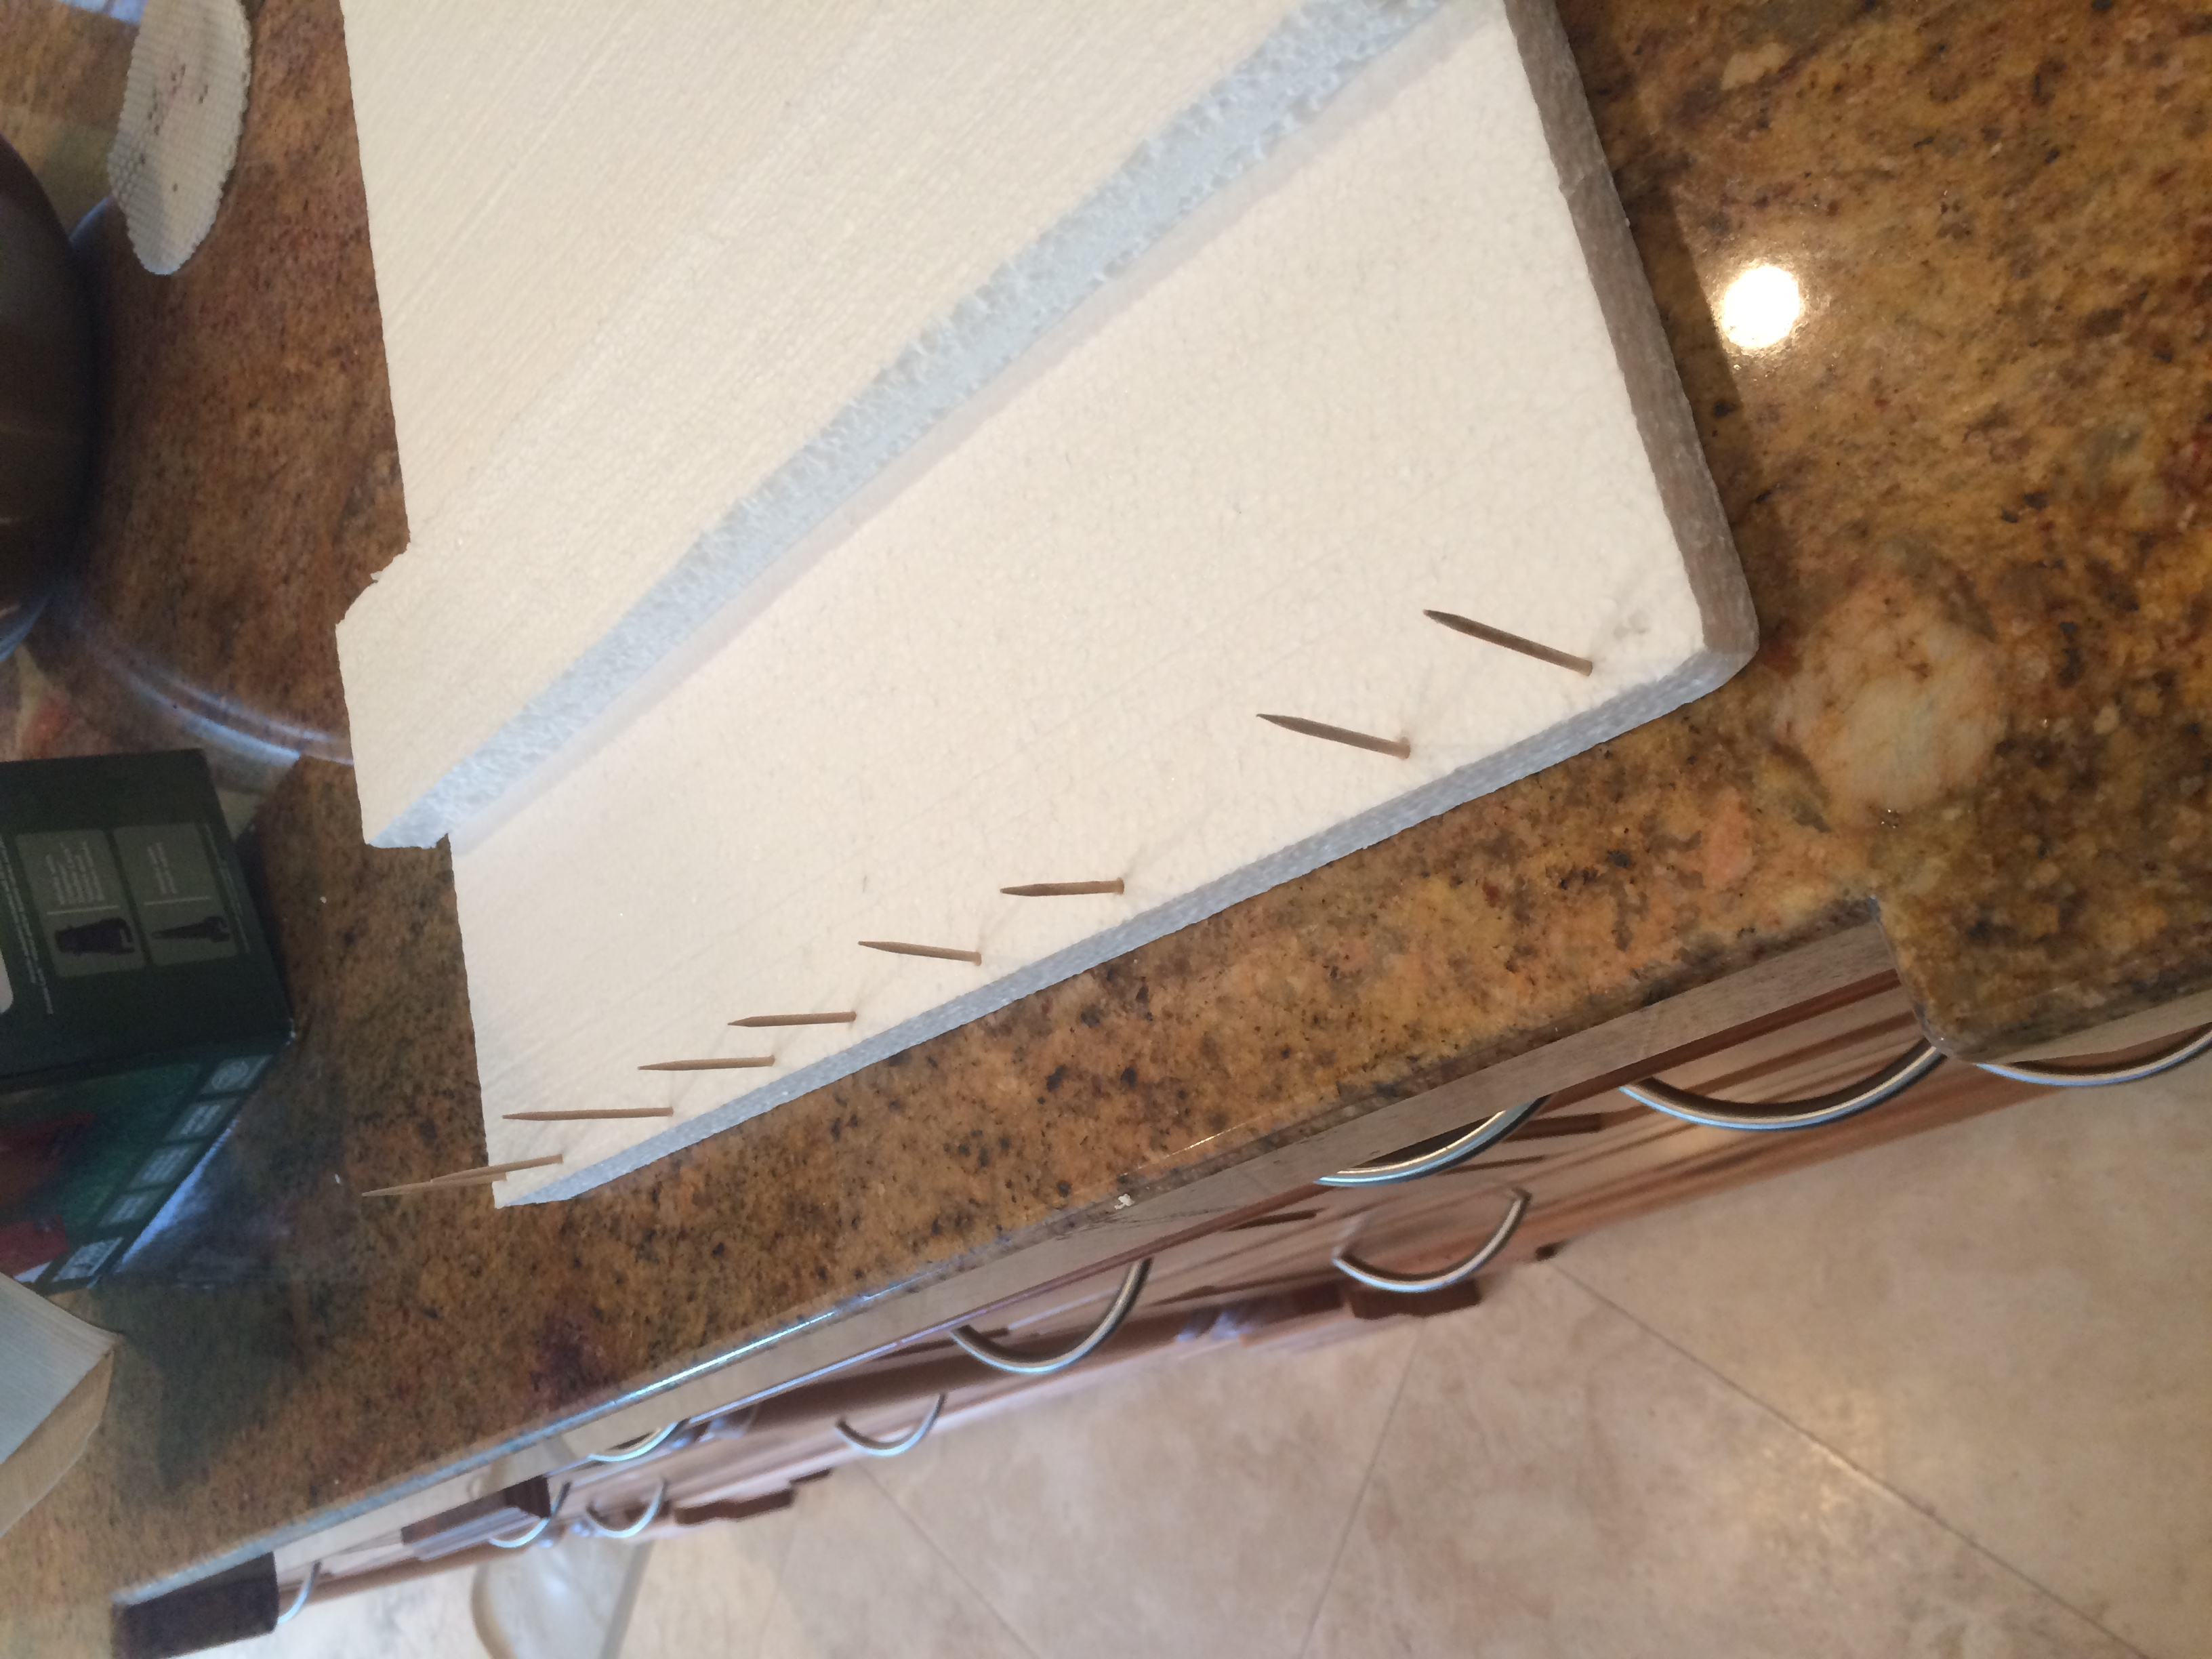
\includegraphics[width=3cm,angle=270]{base_construction}
  \label{fig:sub1}
\end{subfigure}
\begin{subfigure}{.3\textwidth}
  \centering
  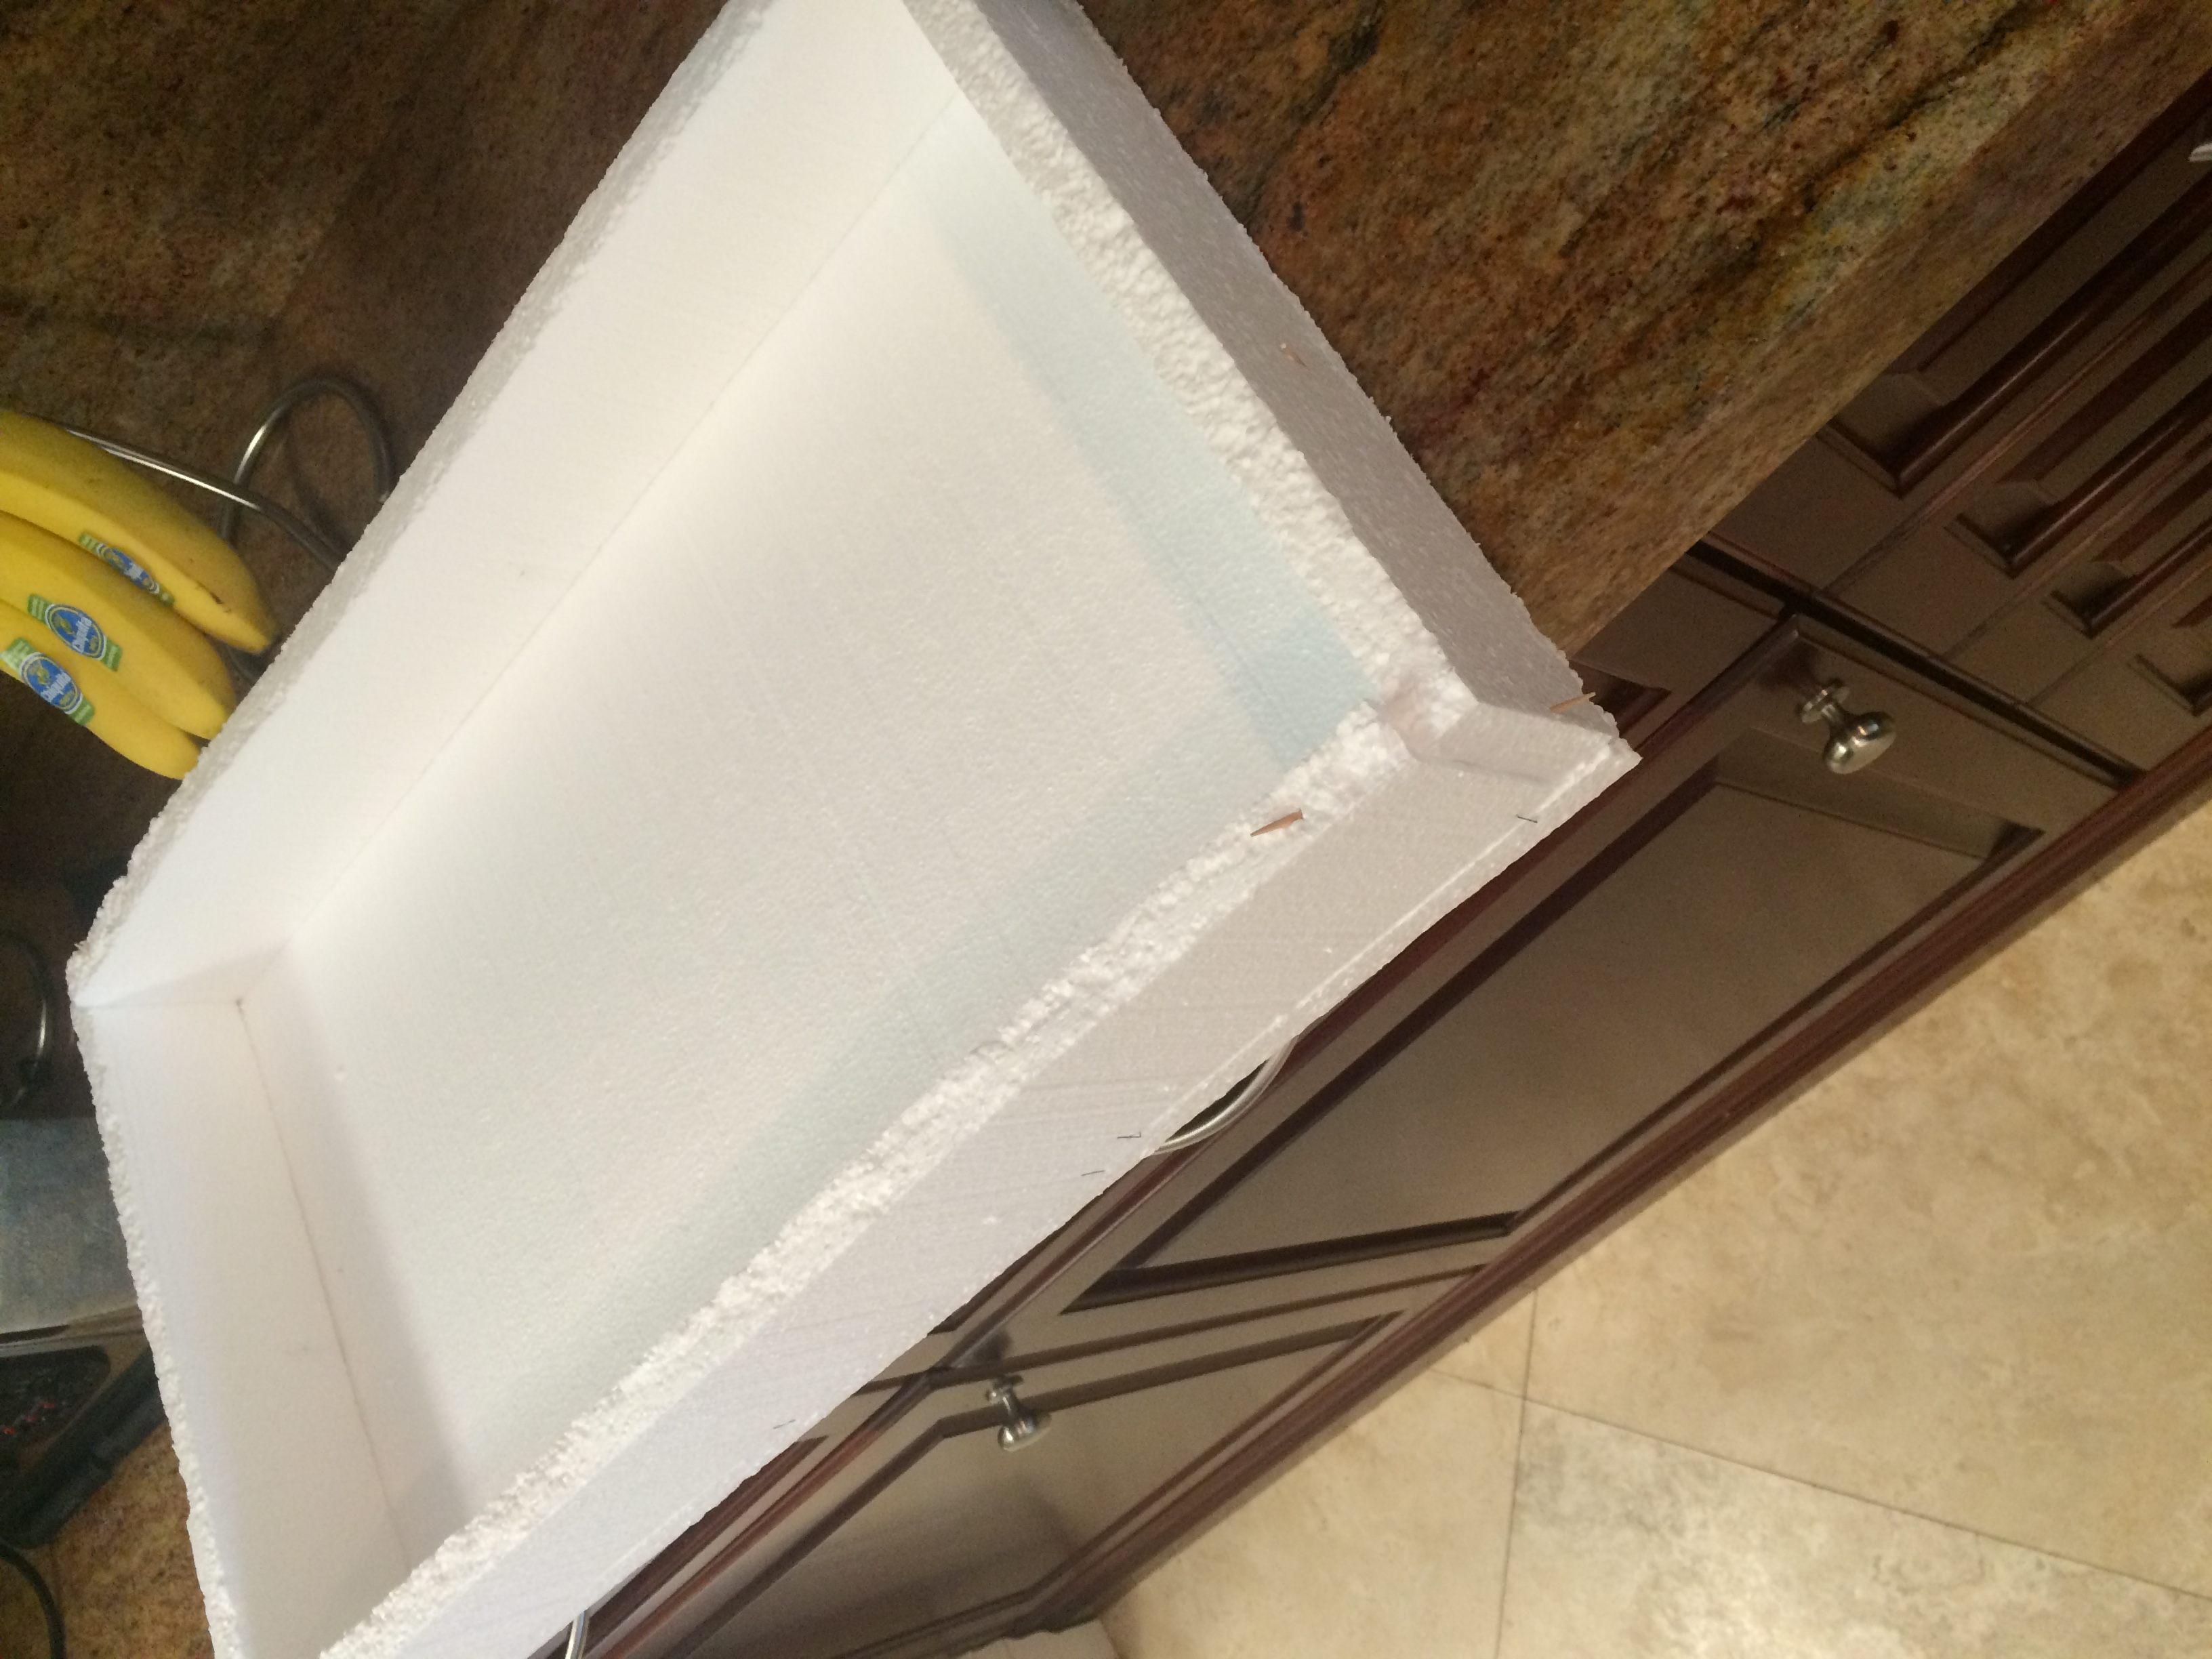
\includegraphics[width=3cm,angle=270]{base_construction_2}
  \label{fig:sub2}
\end{subfigure}
\begin{subfigure}{.3\textwidth}
  \centering
  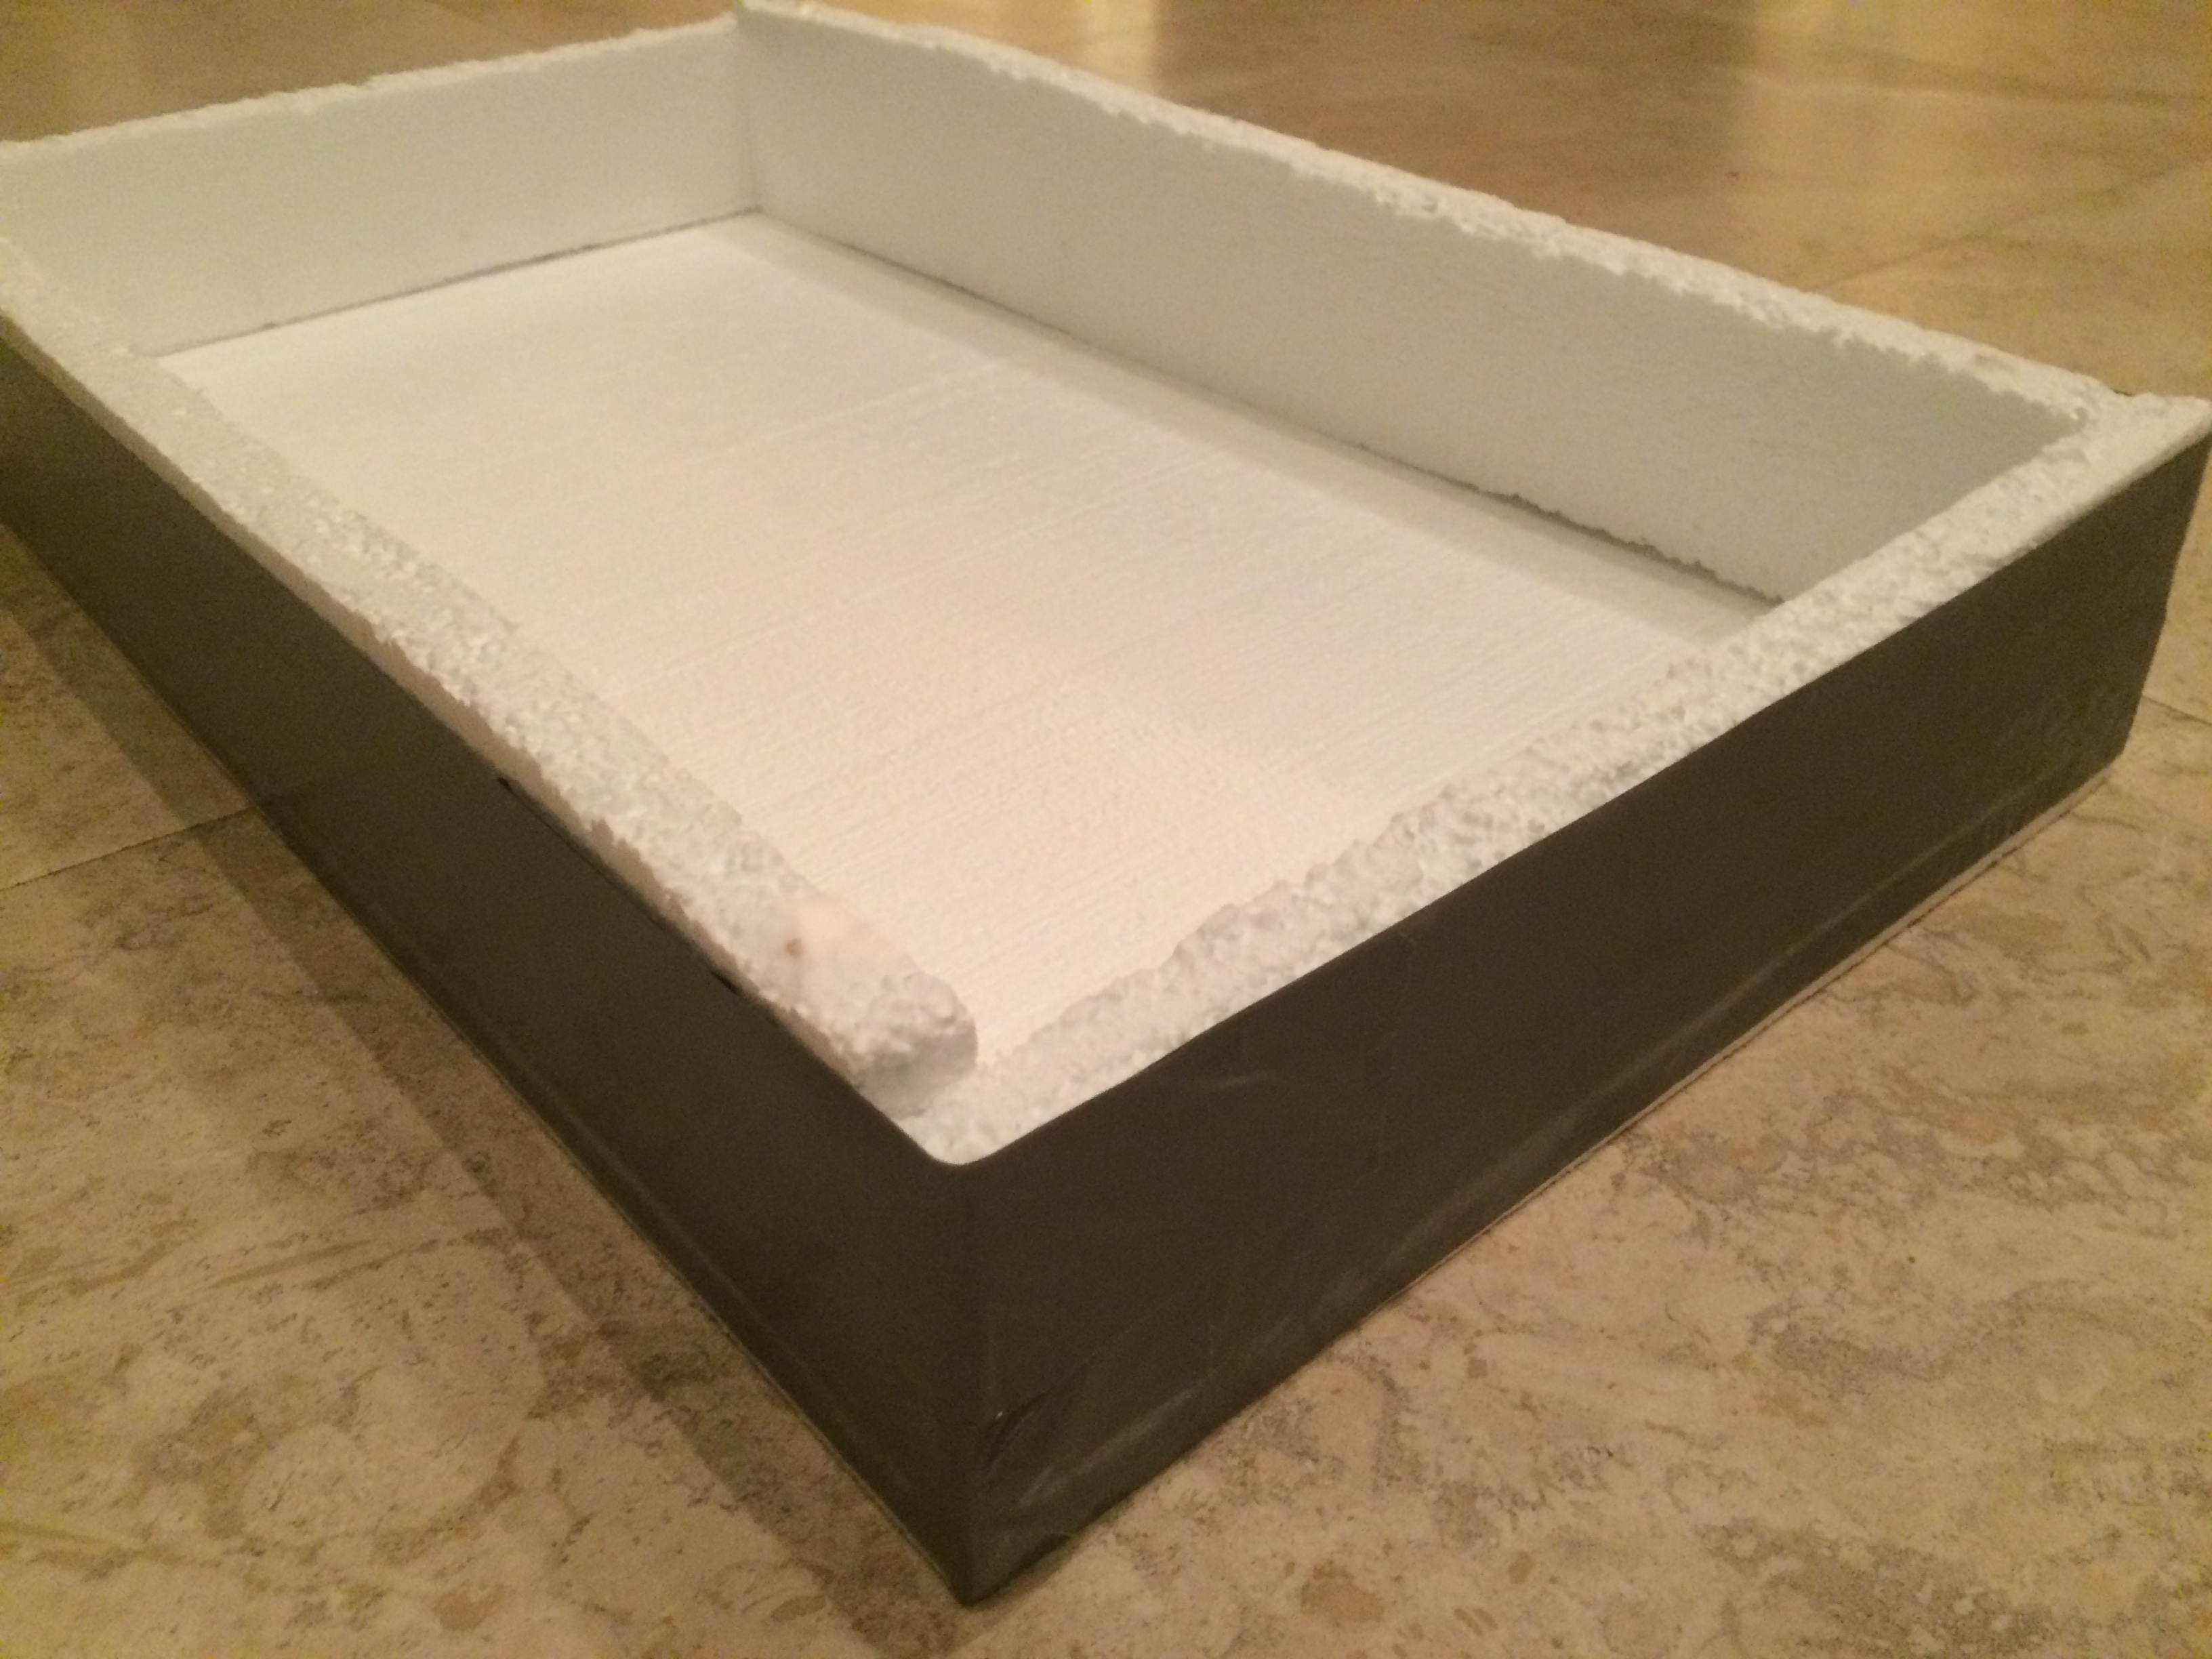
\includegraphics[width=3cm]{base}
  \label{fig:sub2}
\end{subfigure}
\label{fig:test}
\end{figure}

\begin{figure}
\centering
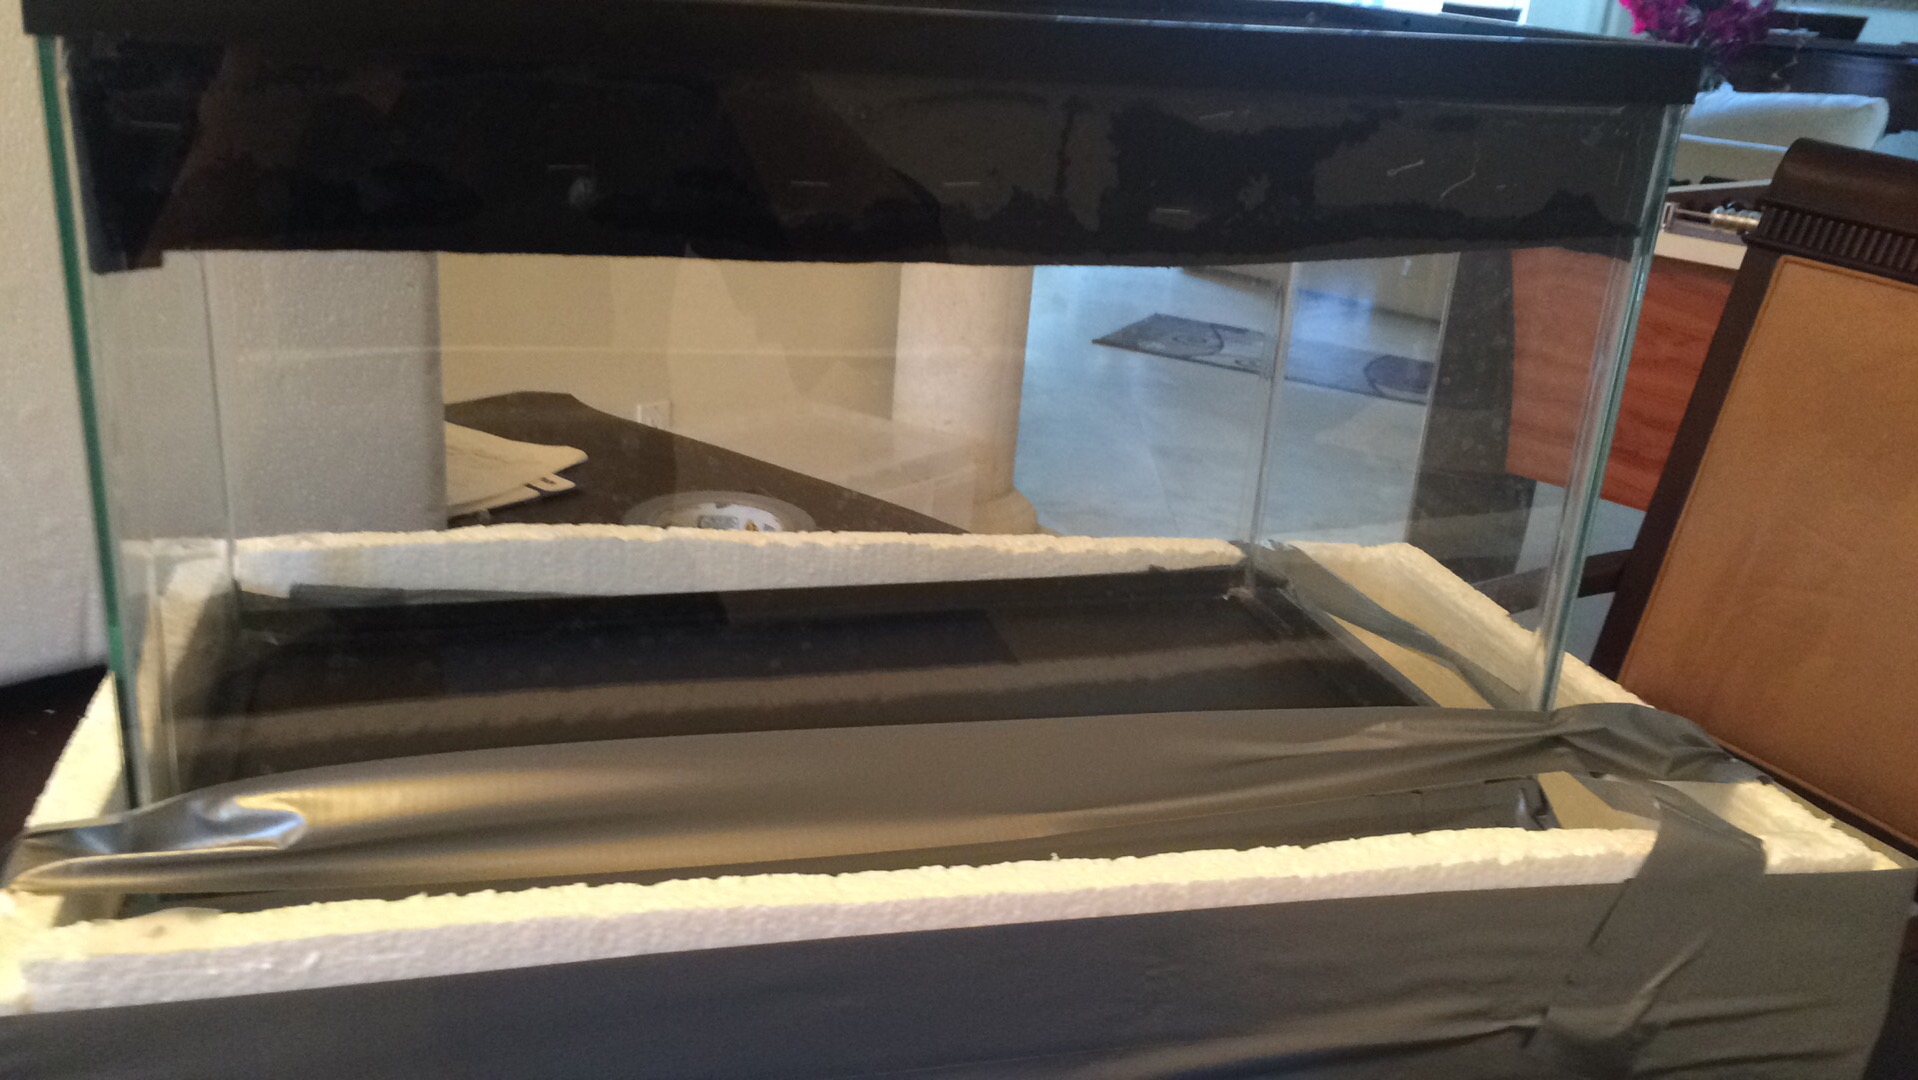
\includegraphics[width=0.5\textwidth]{assembled}
\end{figure}

Running the chamber required planning, timing and careful setup. I first purchased 2 bags (\$15-20 total) of dry ice at Publix, bringing them home in a styrofoam cooler. Using gloves, I laid the sheets of ice inside my styrofoam tub, making sure to fully cover the bottom of the chamber. I soaked the black felt with around 300 mL of isopropyl alcohol; duct-taped the base to the open end of the aquarium, making sure it was airtight; and turned the sealed chamber upside-down on top of the dry ice. The ice was slippery, so I secured the chamber in place with more duct tape. Finally, I shined a flashlight into the side of the chamber near the bottom, held steady with duct tape.

It took approximately 15 minutes for the bottom track-forming region (around 2 cm in height) to get cold enough for the supercooled vapor to form.  The tracks were visible from most angles around the chamber, a benefit of using a glass-walled aquarium. It was easier to see the tracks from the side, but logistically it was better to take pictures and video of the tracks from the top. The tracks formed slowly initially, but within a couple of hours, there was steady and frequent production. The chamber could have run as long as the temperature differential was maintained and alcohol remained in the felt.  After a successful 10 hour run, neither the dry ice nor the alcohol was close to running out.

In total, I collected around 5 hours of video to process.  I used an HD handheld camcorder resting on top of the chamber looking down through the glass to record, giving me 1920x1080 pixel video at 30fps.  The videos were taken in a completely dark room to ensure constant light levels and a more constant background.  

\section{Track Detection}

The track video processing code is written in Python 2.7 using the \texttt{opencv3} and \texttt{numpy} libraries.  For each frame of the video, it follows a number of steps:
\begin{enumerate}
	\item Filter out the background from the frame
	\item Process the mask to remove artifacts
	\item Find groups of remaining pixels
	\item Merge nearby groups
	\item Fit a line to each group
	\item Match each line with similar lines from the previous frame
\end{enumerate}

And after the video has been processed, it follows a second process to record the events:
\begin{enumerate}
	\setcounter{enumi}{6}
	\item Filter out short-lived spurious lines
	\item Enter remaining lines as particle events
\end{enumerate}

\subsection{Filter out the background from the frame}

A typical frame of the video looks like Figure~\ref{fig:frame}.

\begin{figure}[h]
	\centering
	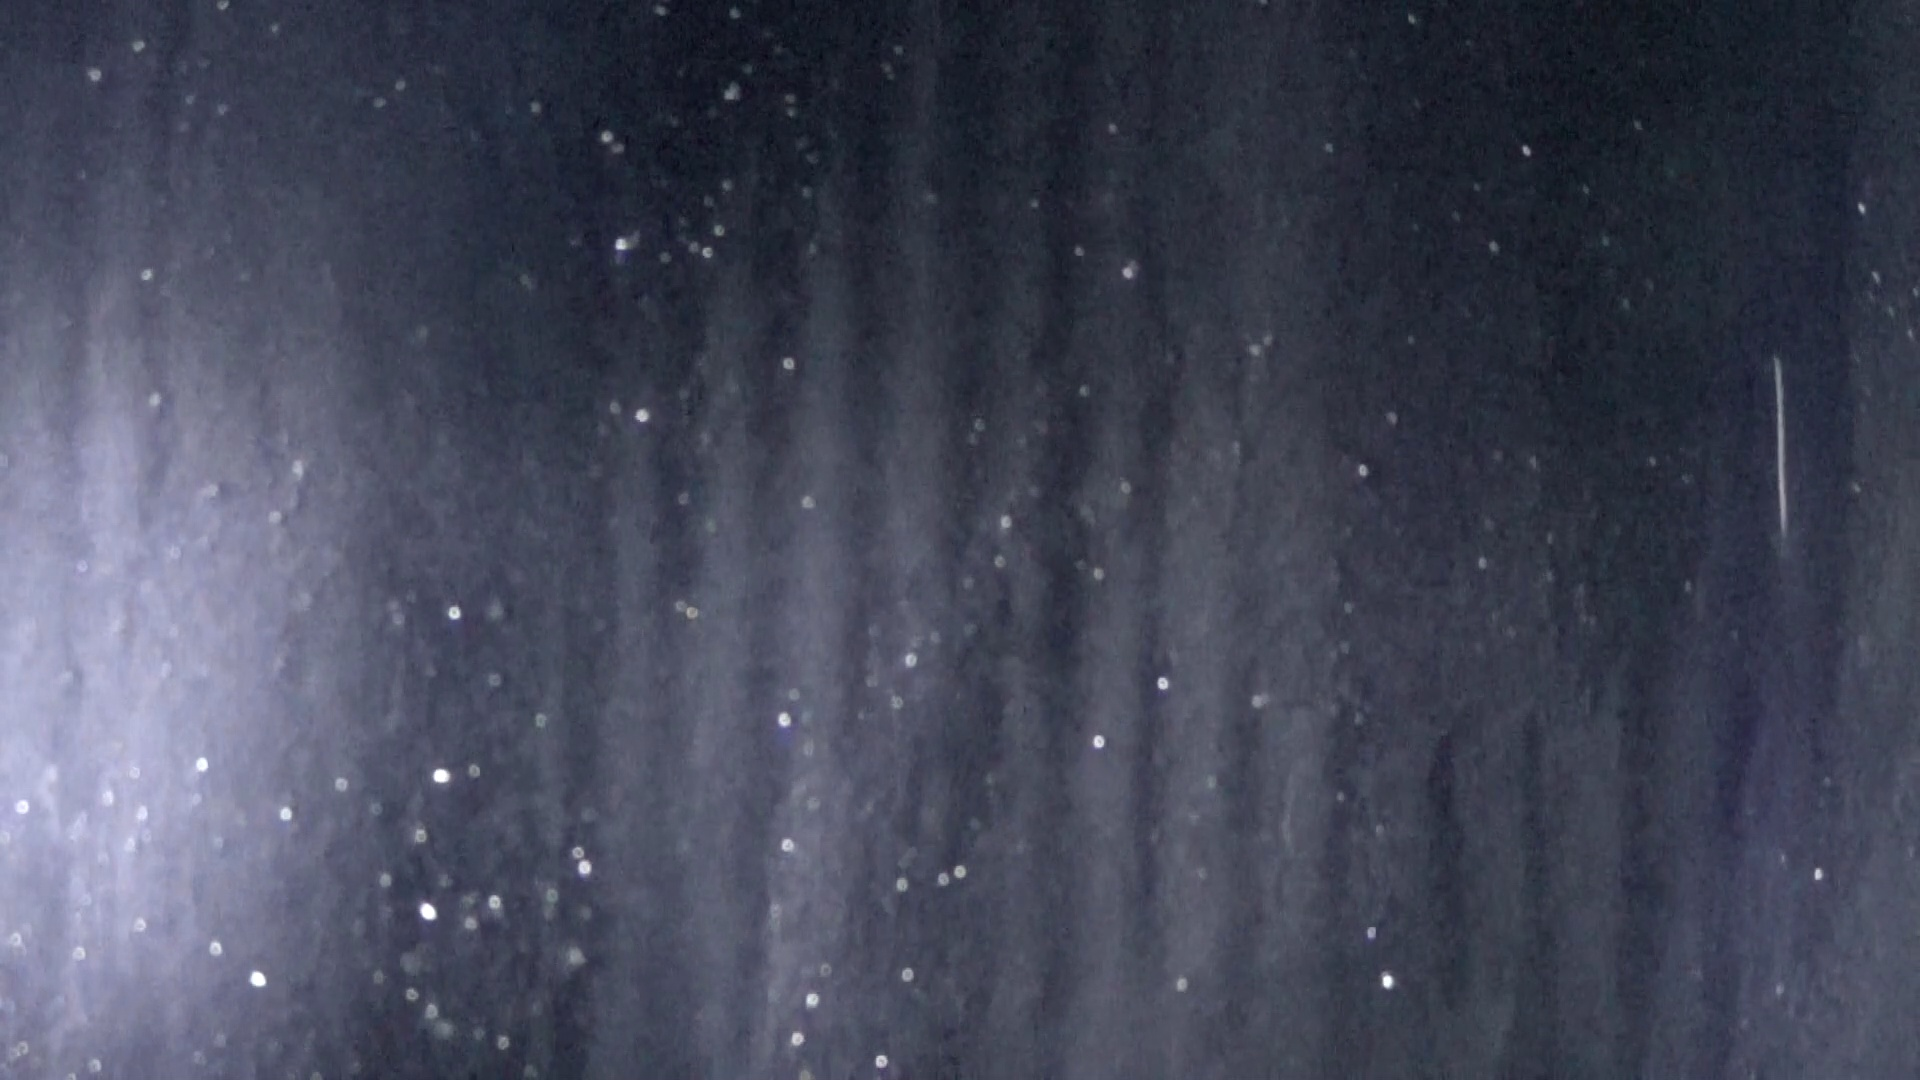
\includegraphics[width=.45\textwidth]{frame}
	\caption{A frame of the video\label{fig:frame}}
\end{figure}

There is a clearly visible track on the right side of the image, but there are also two other fainter tracks at the bottom left that are not visible in a still frame.  Nevertheless, the algorithm will catch them.

Background filtering is done with OpenCV's MOG2 background subtractor.  The filter is initialized with:
\begin{lstlisting}
fgbg = cv2.createBackgroundSubtractorMOG2()
fgbg.setVarThreshold(30)
\end{lstlisting}
and the actual filtering is done with 
\begin{lstlisting}
mask = fgbg.apply(img)
\end{lstlisting}

The mask now looks like Figure~\ref{fig:mask1}, and you can now see the two smaller tracks at the bottom-left.

\begin{figure}[h]
	\centering
	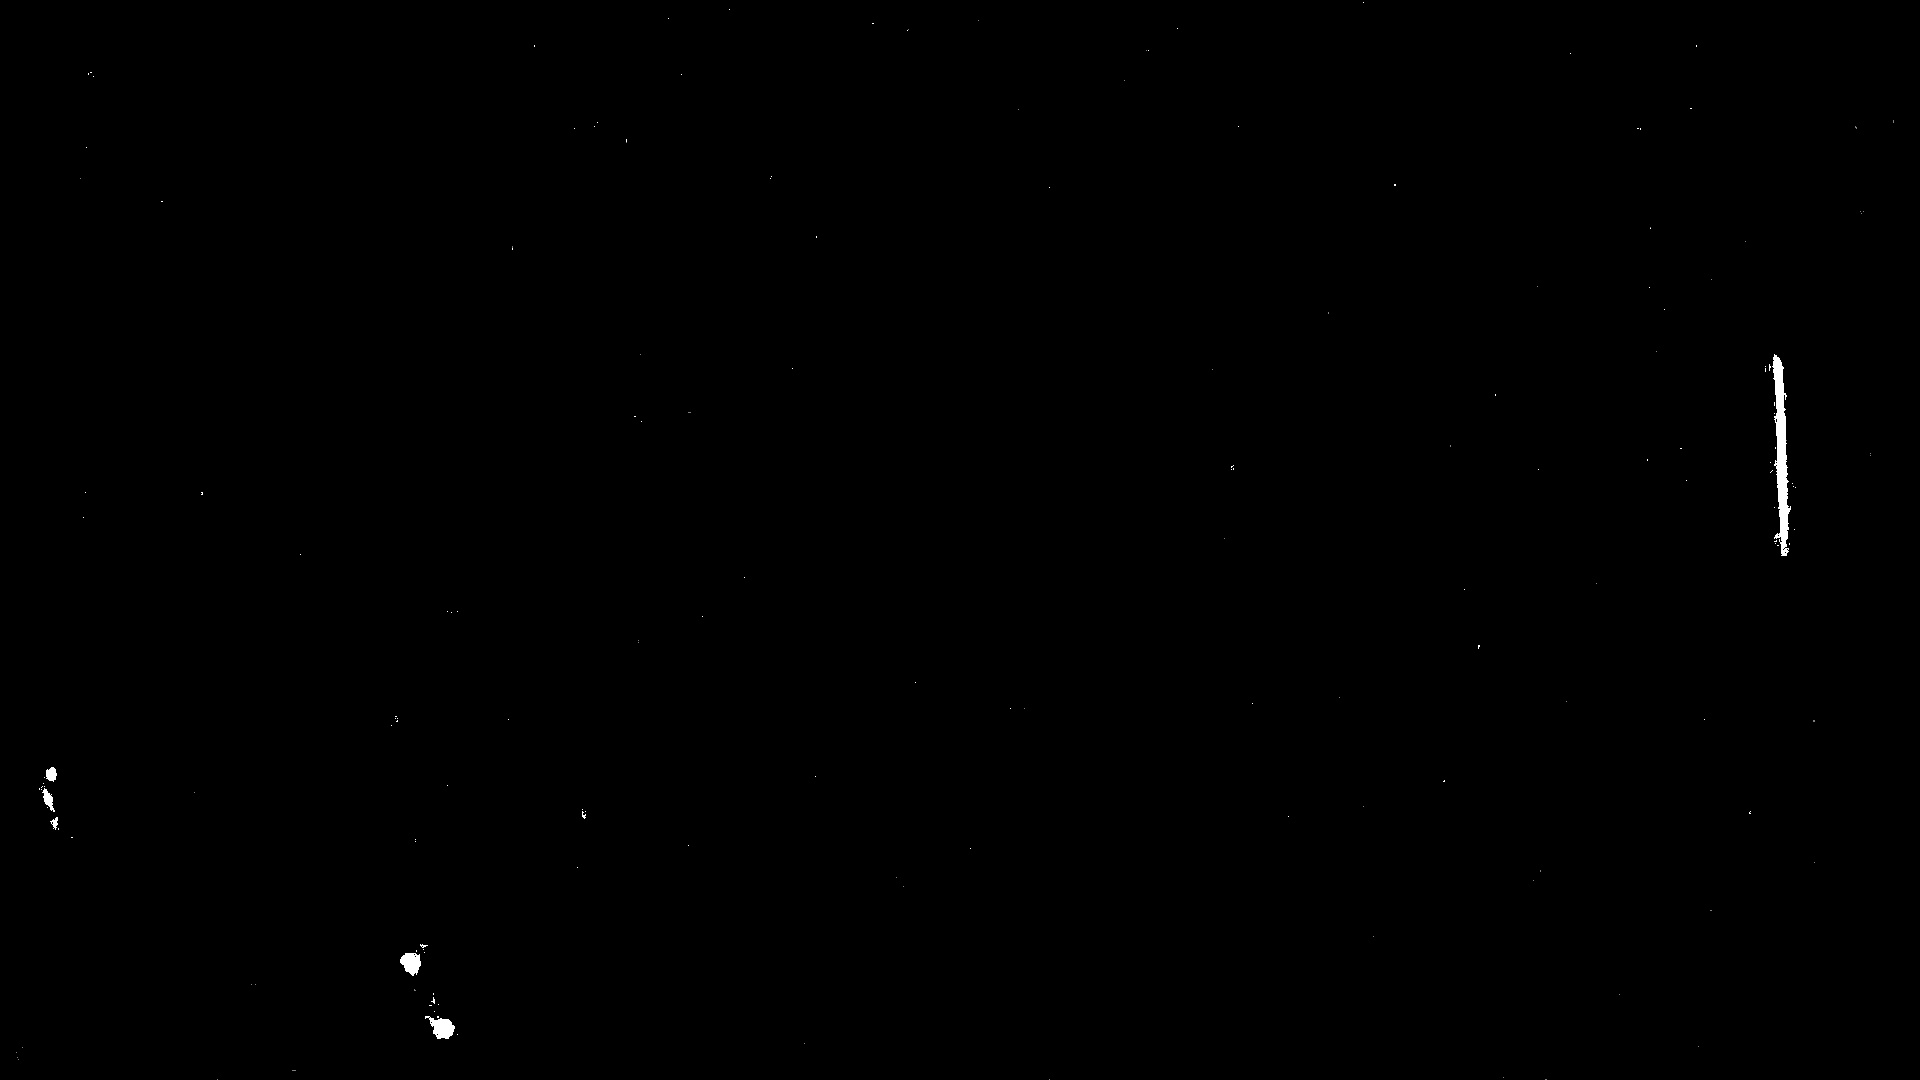
\includegraphics[width=.45\textwidth]{mask1}
	\caption{Background mask}
	\label{fig:mask1}
\end{figure}

\subsection{Process the mask to remove artifacts}
The foreground mask contains many small, 1-2 pixel artifacts, visible as static on the mask.  These are caused by a variety of sources: random lighting changes, camera noise, and drifting chamber fog.  These are filtered out with a blur, then a threshold to isolate large features:
\begin{lstlisting}
mask = cv2.blur(mask, (15, 15))
ret, mask = cv2.threshold(mask, 64, 255, cv2.THRESH_BINARY)
\end{lstlisting}
and then the remaining features, all possible tracks, are enlarged to compensate for the blur:
\begin{lstlisting}
mask = cv2.dilate(mask, (4,4))
\end{lstlisting}
The filtered mask can be seen in Figure~\ref{fig:mask2}.

\begin{figure}[h]
	\centering
	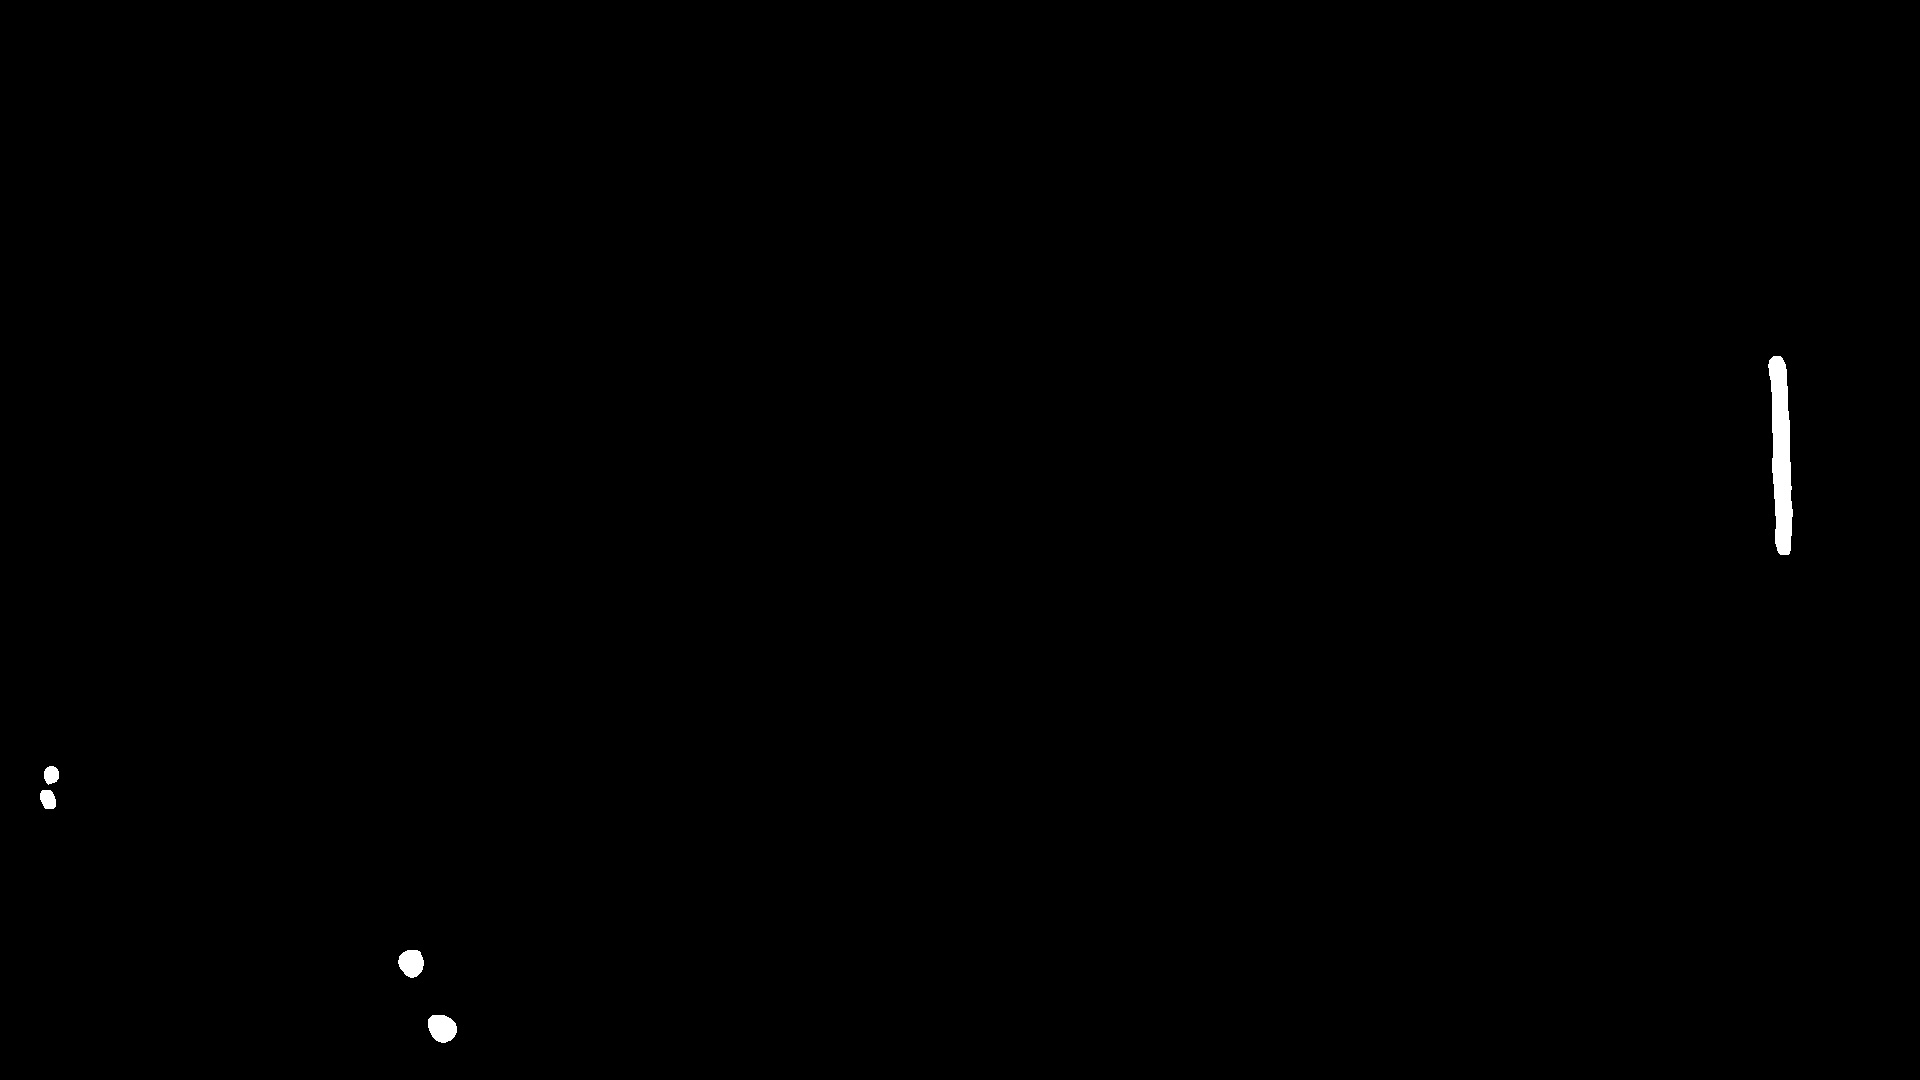
\includegraphics[width=.45\textwidth]{mask2}
	\caption{Mask after artifact removal\label{fig:mask2}}
\end{figure}

\subsection{Find groups of remaining pixels}
I tried many methods to detect lines in the features in the generated mask, including Canny edge detection, Hough transforms, and simple statistical regression, but what ended up working was a simpler, hacked-together method of bounding boxes and contours, which occupies the next three steps in the video algorithm.

The first step in this process is to find groups of pixels in the generated mask, which correspond to events. This is first done with OpenCV's \texttt{findContours} method:
\begin{lstlisting}
i, contours, hierarchy = \
	cv2.findContours(mask, cv2.RETR_TREE, \
	    cv2.CHAIN_APPROX_SIMPLE)
\end{lstlisting}

However, oftentimes single tracks in the video are broken up into multiple separated pixel groups by the blur-threshold process.  Therefore, if we find more than one contour in each mask, we need to join together close contours:
\begin{lstlisting}
if contours and len(contours) > 1:
	contours = join_contours(contours)
\end{lstlisting}

Figure~\ref{fig:mask3} is the mask with contours highlighted, and as you can see the lowest track has been turned into two contours.

\begin{figure}[h]
	\centering
	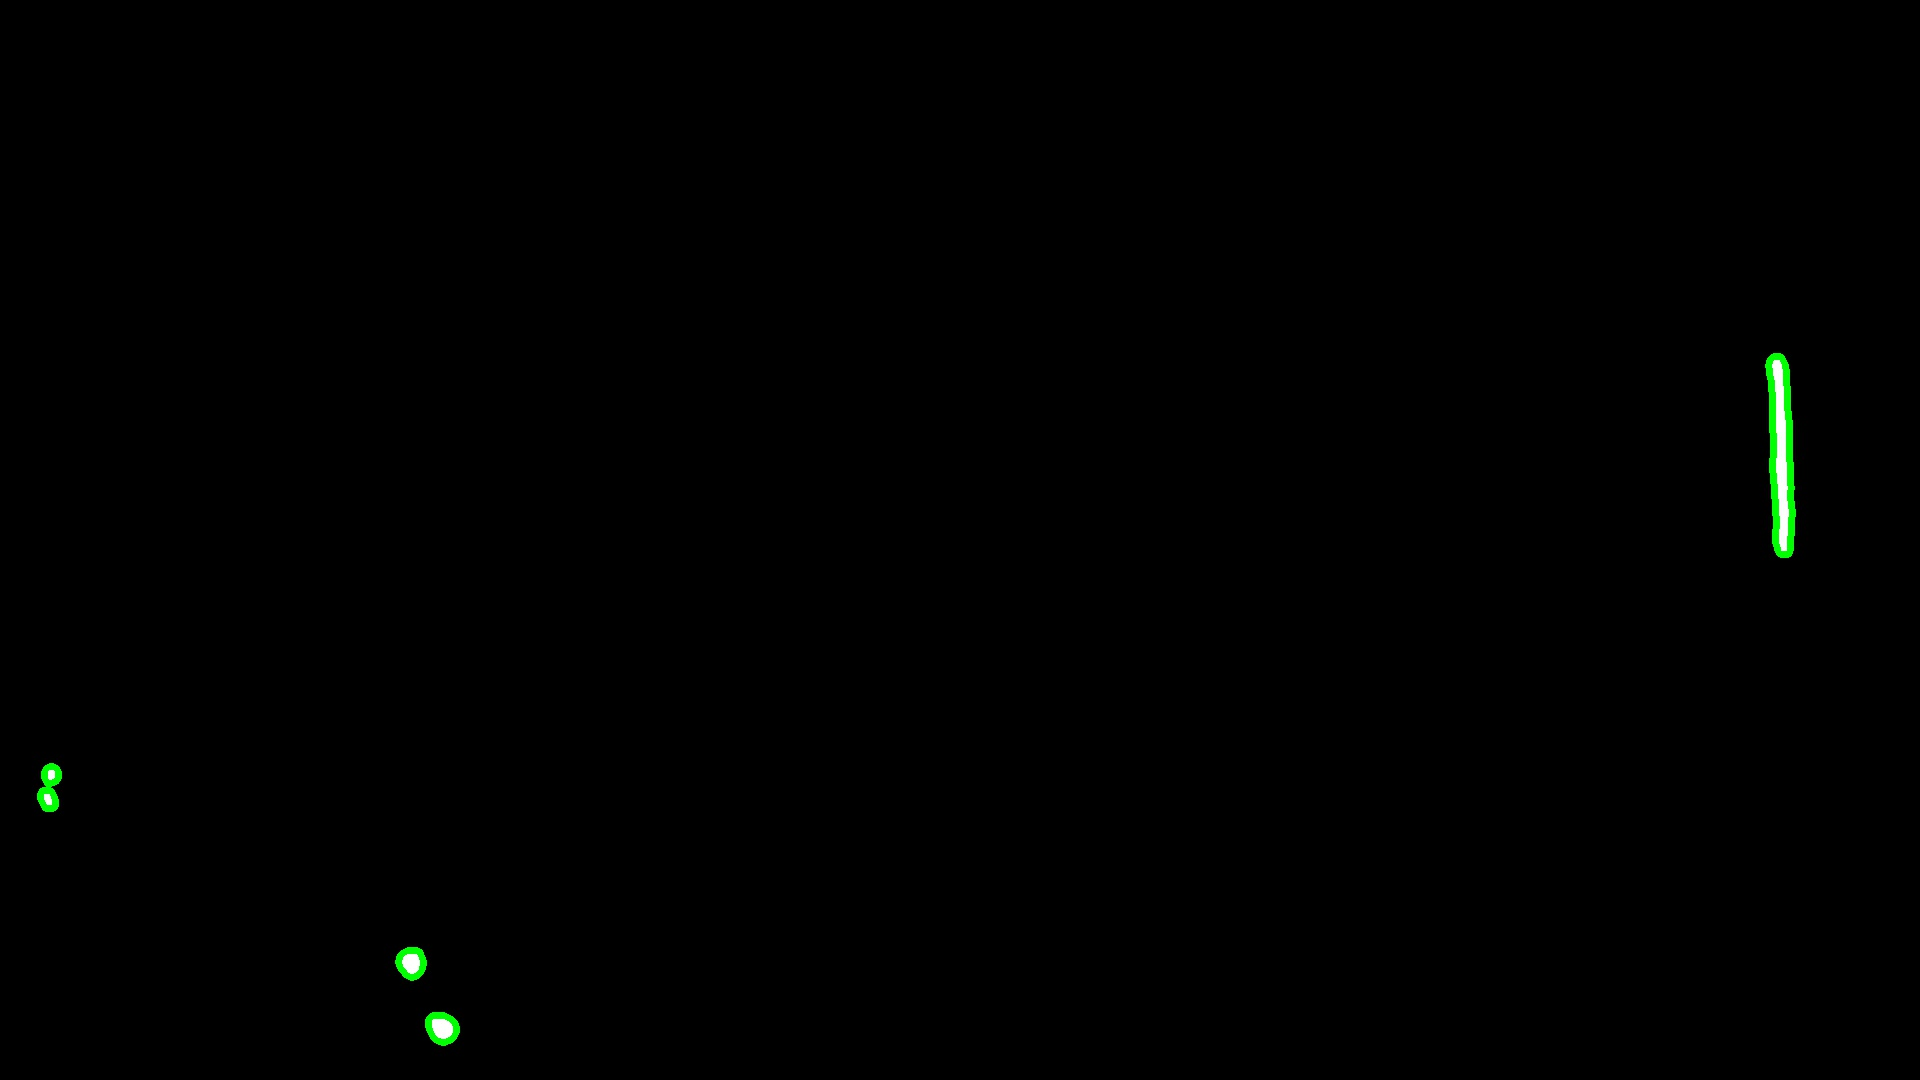
\includegraphics[width=.45\textwidth]{mask3}
	\caption{Mask after \texttt{findContours}\label{fig:mask3}}
\end{figure}

\subsection{Merge nearby groups}

\texttt{join\_contours} is a long Python method which iterates through each contour, finding its close neighbors, then finally joins each set of close contours.  It is based on code found at \cite{join}.


It requires \texttt{find\_if\_close}, which determines if two contours come within 100 pixels of each other by comparing the distance between their points:
\begin{lstlisting}
def find_if_close(cnt1, cnt2):
    row1, row2 = cnt1.shape[0], cnt2.shape[0]
    for i in xrange(row1):
        for j in xrange(row2):
            dist = np.linalg.norm(cnt1[i]-cnt2[j])
            if abs(dist) < 100 :
                return True
            elif i == row1-1 and j == row2-1:
                return False
\end{lstlisting}

Now we are ready to begin \texttt{join\_contours}:
\begin{lstlisting}
def join_contours(contours):
\end{lstlisting}

\texttt{join\_contours} keeps its data in a \texttt{status} array, which for each contour represents the lowest ID among its neighbors:
\begin{lstlisting}
    LENGTH = len(contours)
    status = np.zeros((LENGTH,1))
\end{lstlisting}

Now \texttt{join\_contours} iterates through each contour, and for each contour it finds all (non-processed) neighbors and stores their relationship in \texttt{status}:
\begin{lstlisting}
    for i, cnt1 in enumerate(contours):
        x = i    
        if i != LENGTH-1:
            for j,cnt2 in enumerate(contours[i+1:]):
                x = x+1
                dist = find_if_close(cnt1,cnt2)
                if dist == True:
                    val = min(status[i],status[x])
                    status[x] = status[i] = val
                else:
                    if status[x]==status[i]:
                        status[x] = i+1
\end{lstlisting}

Finally, \texttt{join\_contours} merges all of the contours that share the same \texttt{status} ID:
\begin{lstlisting}
    unified = []
    maximum = int(status.max())+1
    for i in xrange(maximum):
        pos = np.where(status==i)[0]
        if pos.size != 0:
            cont = np.vstack(contours[i] for i in pos)
            hull = cv2.convexHull(cont)
            unified.append(hull)

    return unified
\end{lstlisting}

After \texttt{join\_contours}, Figure~\ref{fig:mask4} is what the mask looks like; note that the two contours on the lowest track have been joined.

\begin{figure}[h]
	\centering
	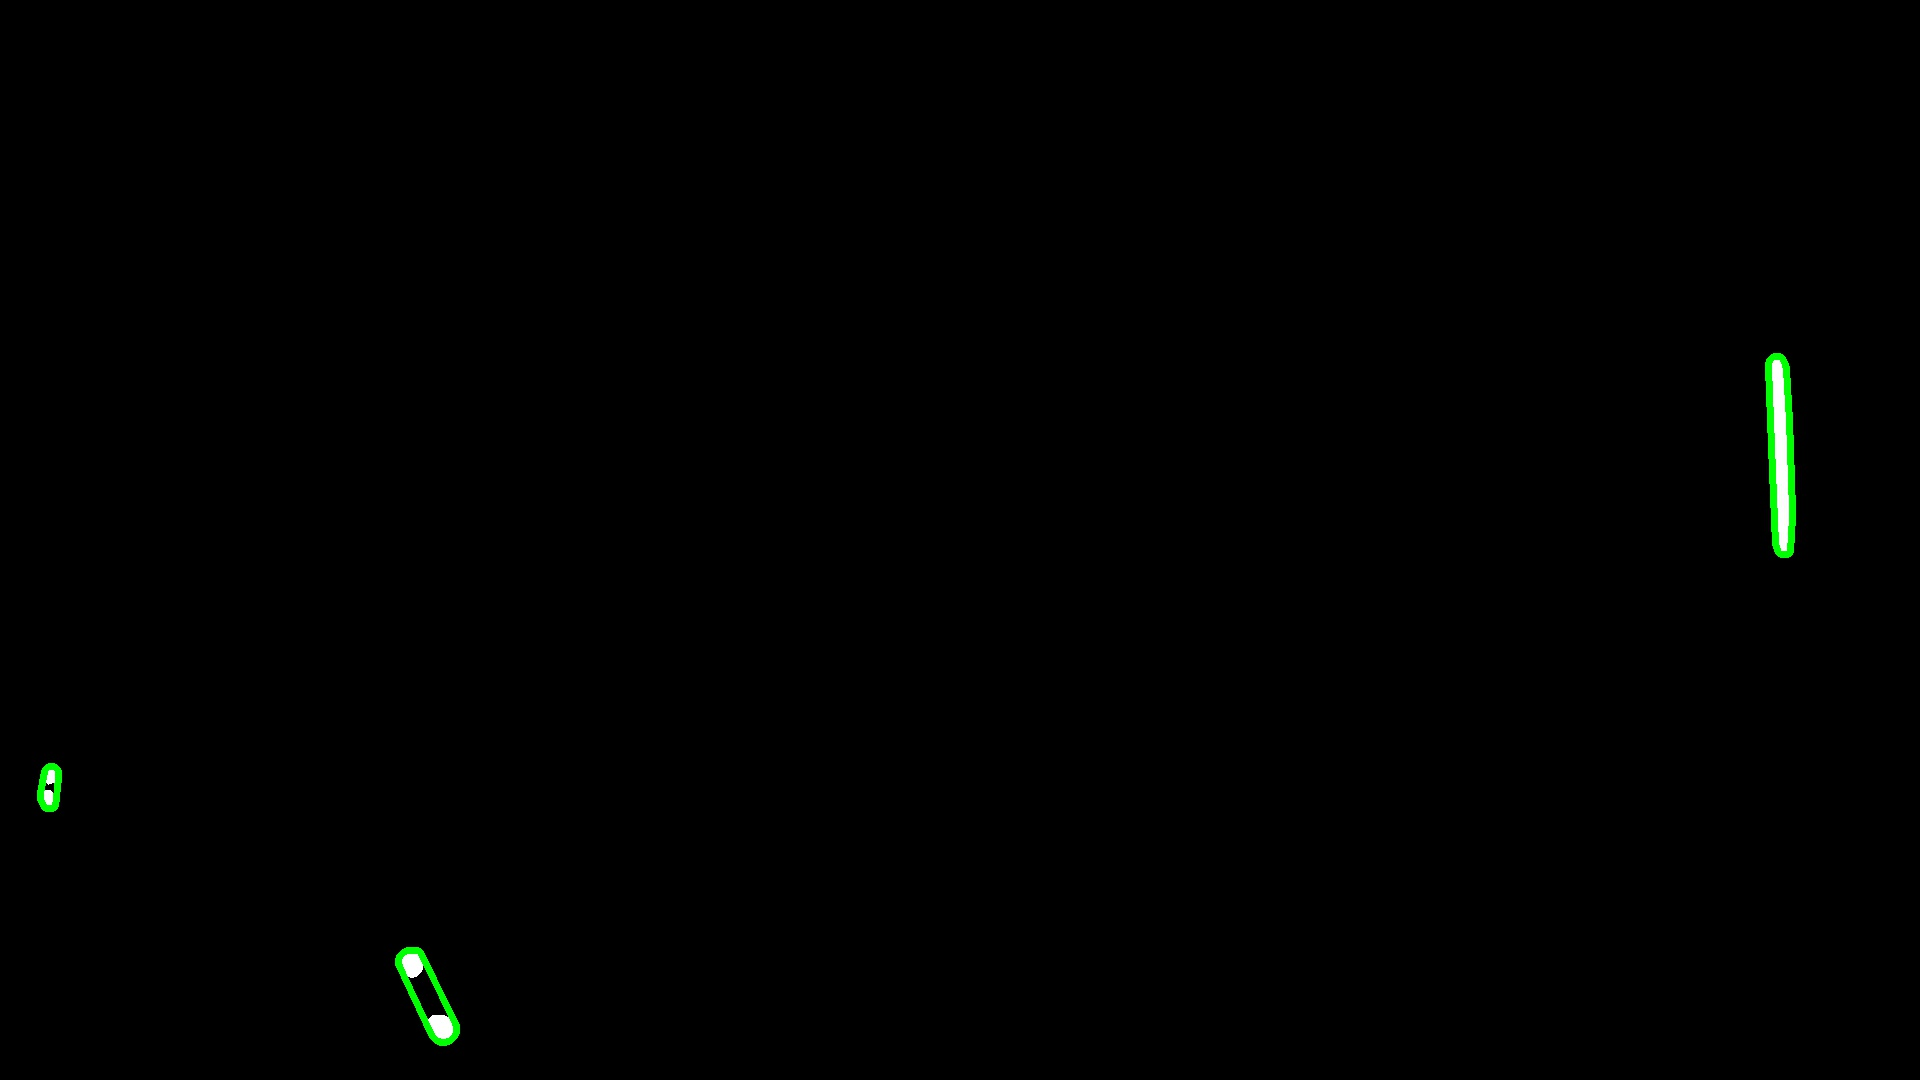
\includegraphics[width=.45\textwidth]{mask4}
	\caption{Mask after \texttt{joinContours}\label{fig:mask4}}
\end{figure}

\subsection{Fit a line to each group}

Once all of the points in a single track have been identified, we can now fit a line to them.  I decided on a simple method, just fitting a bounding rotated rectangle to the points; the major axis of the rectangle is a reasonable approximation of the underlying track.

First we find a bounding rotated rectangle:
\begin{lstlisting}
    center, sides, angle = cv2.minAreaRect(contour)
    x, y = center
    l, m = sides
    theta = np.radians(angle)
\end{lstlisting}

Next, we find the start and end coordinates of the underlying line, through a little trigonometry:
\begin{lstlisting}
    if l > m:
        a = (int(x - l*np.cos(theta)), int(y - m*np.sin(theta)))
        b = (int(x + l*np.cos(theta)), int(y + m*np.sin(theta)))
    else:
        a = (int(x - m*np.sin(theta)), int(y + m*np.cos(theta)))
        b = (int(x + m*np.sin(theta)), int(y - m*np.cos(theta)))
\end{lstlisting}

The identified tracks are shown in Figure~\ref{fig:mask5}.

\begin{figure}[h]
	\centering
	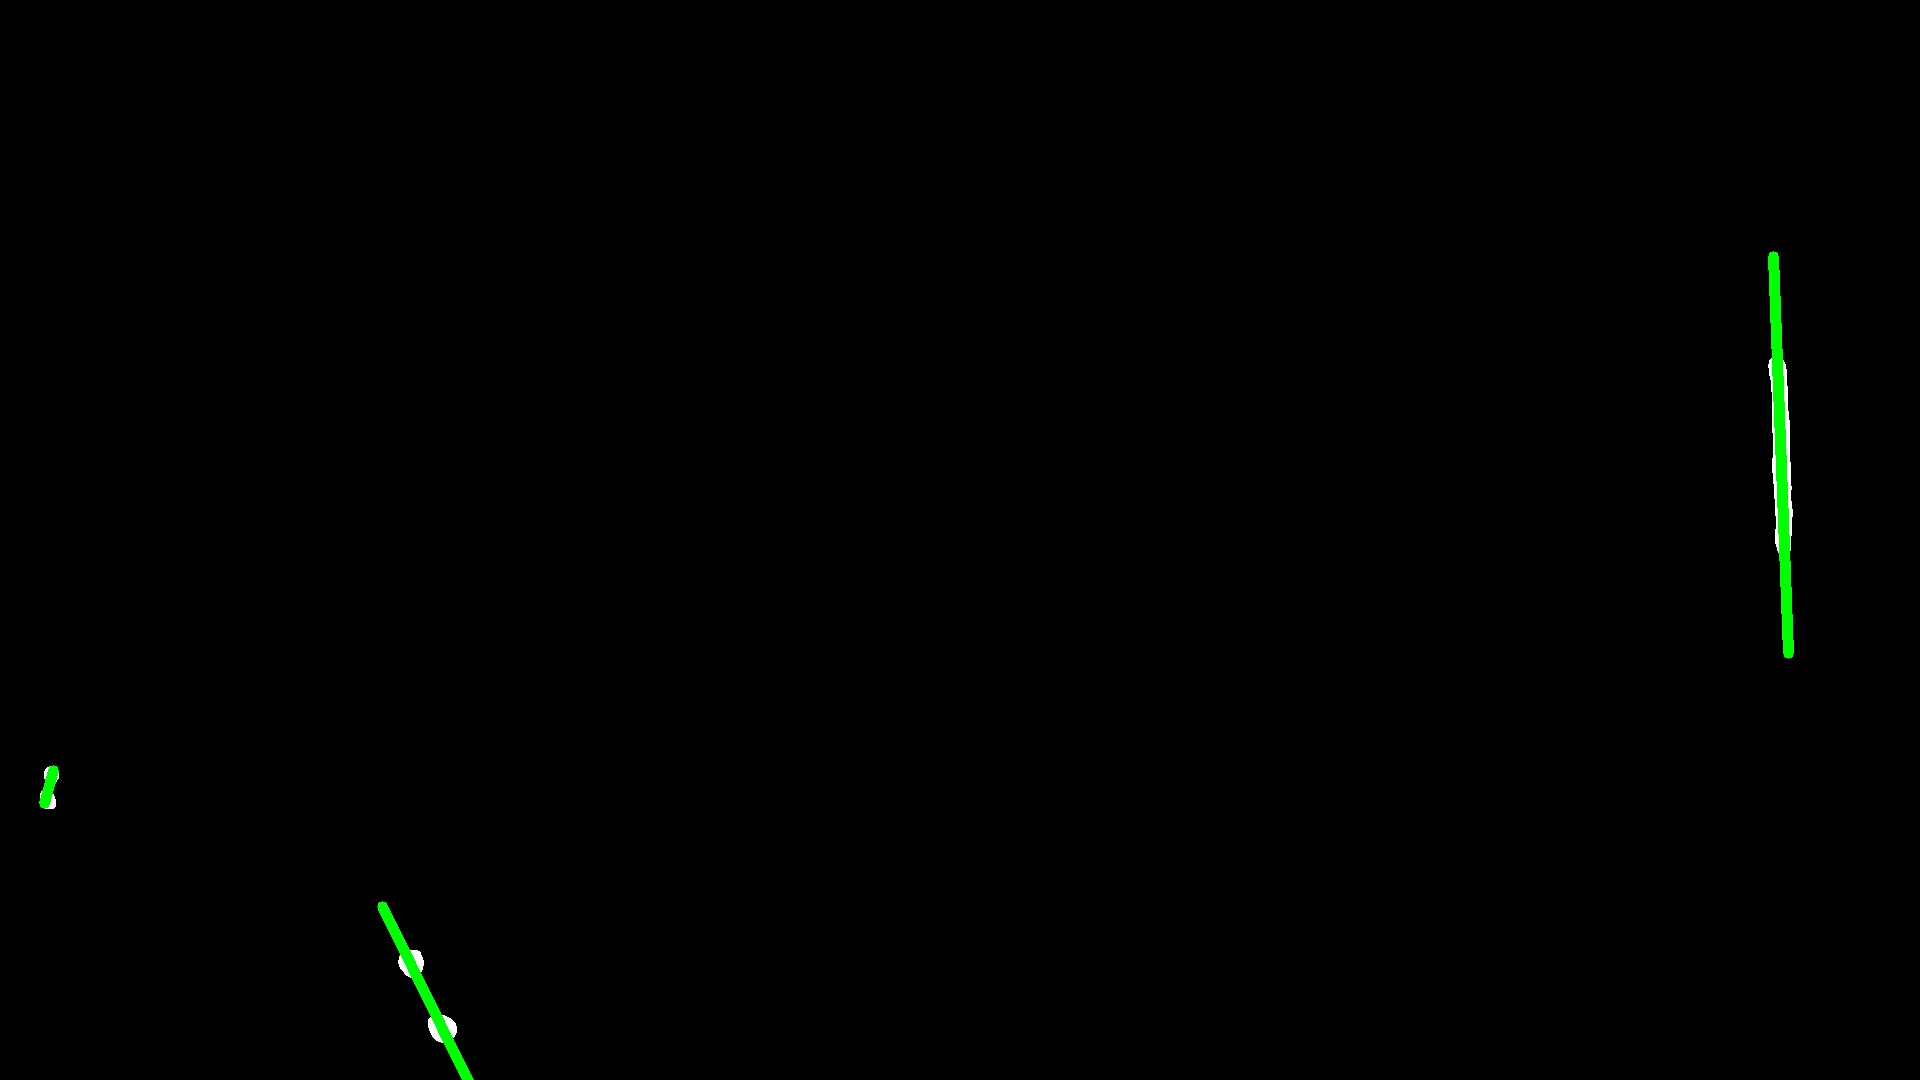
\includegraphics[width=.45\textwidth]{mask5}
	\caption{Tracks identified\label{fig:mask5}}
\end{figure}

Now we can extract properties about the track, like its length, brightness, and divergence from linearity.

Its length is a simple calculation, just the distance between the two endpoints of the line:
\begin{lstlisting}
    length = np.linalg.norm(np.array(a)-np.array(b))
\end{lstlisting}    

The track intensity, however, is a bit more complicated.  I approximate it by finding the number of activated pixels in the group and dividing by the track's bounding area, sort of a brightness/unit calculation.  These intensities are not in an objective unit scheme, but are relative.  In general, alpha particles will have a higher calculated intensity (because they are brighter and straighter), while beta particles will have a lower calculated intensity.

To calculate this quantity, I first isolate the portion of the mask that is relevant:
\begin{lstlisting}
    matrix = cv2.getRotationMatrix2D(center, angle, 1)
    rotated = cv2.warpAffine(mask, matrix, mask.shape[:2])
    rect = cv2.getRectSubPix(rotated, (int(l),int(m)), center)
\end{lstlisting}    
and then count the non-zero pixels in that area:
\begin{lstlisting}
    intensity = float(cv2.countNonZero(rect))/(l*m)
\end{lstlisting}    

The divergence of the track has been totally ignored thus far (since we assume a linear track when we find a line using a bounding rectangle), but we can somewhat quantify it as the rotated rectangle's aspect ratio.  This is either \texttt{l/m} or \texttt{m/l}, but it's also the area of the rectangle over the the square of its major axis:
\begin{lstlisting}
    divergence = (l*m)/(length*length)
\end{lstlisting}
    
We now have each track's angle of incidence, intensity, length, divergence, and endpoints.

\subsection{Match each line with similar lines from the previous frame}

Instead of collecting all lines and collating them into events at the end of processing, the program collates them as the video is processed.  This is done through two global dictionaries, \texttt{events} tracking collated events and \texttt{eventlist} tracking uncollated lines:
\begin{lstlisting}
eventlist = {}
events = {}
\end{lstlisting}    
the frame-local array \texttt{currentevents} tracking the lines in the current frame:
\begin{lstlisting}
currentevents = []
\end{lstlisting}    
the global \texttt{nextid}, tracking event IDs:
\begin{lstlisting}
nextid = 0
\end{lstlisting}    
and the global \texttt{time}, which counts frames:
\begin{lstlisting}
time = 0
...
time += 1
\end{lstlisting}    

The collation also uses a line-similarity algorithm, \texttt{linesSimilar}.  \texttt{linesSimilar} is a method for comparing if two lines could plausibly be the same.  It checks the difference in their angles:
\begin{lstlisting}
    anglediff = abs(angleA-angleB)
    if anglediff > 30:
        return False
\end{lstlisting}    
and if their endpoints are close together, keeping in mind that the ordering of endpoints in a line is not fixed:
\begin{lstlisting}
    a1 = np.array(la[0])
    a2 = np.array(la[1])
    b1 = np.array(lb[0])
    b2 = np.array(lb[1])
    
    dist1 = np.linalg.norm(a1-b1) > 50
    dist2 = np.linalg.norm(a2-b2) > 50
    dist3 = np.linalg.norm(a1-b2) > 50
    dist4 = np.linalg.norm(a2-b1) > 50
    
    if sum((dist1, dist2, dist3, dist4)) < 2:
        return False
    
    return True
\end{lstlisting}    

On the first frame, each line present in the image is identified as a new event and entered into both \texttt{events} and \texttt{currentevents}, although there are usually no lines:
\begin{lstlisting}
for l in lines:
    currentevents += [(nextid, l)]
    events[nextid] = [(time, l)]
    nextid += 1
\end{lstlisting}    
    
On all other frames, we take each line in turn.  For each line, we search through all lines in the previous frame for a similarity match:
\begin{lstlisting}
for l in lines:
    found = False
    for l2 in eventlist[time-1]:
        if linesSimilar(l, l2[1]):
            currentevents += [(l2[0], l)]
            events[l2[0]] += [(time, l)]
            found = True
            break
\end{lstlisting}    

And if no similar lines are found, we enter the line as a new event:
\begin{lstlisting}
    if not found:
        currentevents += [(nextid, l)]
        events[nextid] = [(time,l)]
        nextid += 1
\end{lstlisting}    

Finally, we add all current lines to \texttt{eventlist} for future comparison:
\begin{lstlisting}
eventlist[time] = currentevents
\end{lstlisting}    

\subsection{Filter out short-lived spurious lines}

All events are now represented in \texttt{eventlist} as a list of lines with an ID.  Unfortunately, some artifacts have been identified as events, as occasionally they get larger than a few pixels.  Fortunately, while true tracks last for a while, artifacts tend to disappear after one or two frames, so we simply filter out the events with short lifespans:
\begin{lstlisting}
events = {k: v for k,v in events.items() if len(v) > 4}
\end{lstlisting}

\subsection{Enter remaining lines as particle events}

I use a MySQL database to store the event records.  The table has this structure:\\

\begin{tabular}{|l|l|}
	\hline
	Field & Type \\ \hline
	\texttt{id} & \texttt{bigint(20) unsigned primary\_key} \\ \hline
	\texttt{angle} & \texttt{double} \\ \hline
	\texttt{length} & \texttt{double} \\ \hline
	\texttt{intensity} & \texttt{double} \\ \hline
	\texttt{timestamp} & \texttt{bigint(20) unsigned} \\ \hline
	\texttt{type} & \texttt{char(1)} \\ \hline
	\texttt{lifespan} & \texttt{int(10) unsigned} \\ \hline
	\texttt{divergence} & \texttt{double} \\ \hline
\end{tabular}
\\[10pt]

\texttt{analyzeEvents} converts between the \texttt{events} structure and the database row structure.  For each event (list of lines), we obtain its event id:
\begin{lstlisting}
event_id = k
\end{lstlisting}
Its timestamp, as the frame number of its first line:
\begin{lstlisting}
timestamp = value[0][0]
\end{lstlisting}
Its age, as the difference between the frame numbers of its first and last lines:
\begin{lstlisting}
age = value[-1][0] - value[0][0]
\end{lstlisting}
To get the rest of the more line-specific values, we extract the list of lines:
\begin{lstlisting}
lines = [l for t,l in value]
\end{lstlisting}
The angle is taken from the 4th line recorded, as a compromise between making sure the entire line has been identified and avoiding recording the natural drift of tracks in the chamber:
\begin{lstlisting}
angle = lines[3][2]
\end{lstlisting}
The length of the track is taken as the 90th percentile of all the lengths of the lines composing it:
\begin{lstlisting}
lengths = np.array([l[4] for l in lines])
length = np.percentile(lengths, 90)
\end{lstlisting}
As is the intensity:
\begin{lstlisting}
intensities = np.array([l[3] for l in lines])
intensity = np.percentile(intensities, 90)
\end{lstlisting}
Track divergence gets bigger as the track drifts, so I take the 20th percentile (to avoid measuring it when the track is really small and difficult to quantify):
\begin{lstlisting}
divergences = np.array([l[5] for l in lines])
divergence = np.percentile(divergences, 20)
\end{lstlisting}
I don't identify the type of particle at this stage, so I record that with a \texttt{"?"}, and the row structure becomes
\begin{lstlisting}
(event_id, angle, length, intensity, timestamp, "?", age, divergence)
\end{lstlisting}
for each event.

I use the \texttt{MySQLdb} library to interface with the database, and because \texttt{analyzeEvents} creates the event listing so nicely, entering the events into the database is a simple loop:
\begin{lstlisting}
for r in rows:
    cursor.execute("INSERT INTO events VALUES "+str(r)+";")
\end{lstlisting}

A final printout gives us the average time per frame to process and the number of events processed.

\subsection{Performance}

I would estimate that the track-finding program has around a 90\% accuracy; it detects nearly all tracks visible, even ones not visible to the human eye on the first viewing of the video, and counts very few artifacts as tracks.  The recorded values for each track have a much lower accuracy; in particular, the length of a track is usually only accurate to within 100 pixels or so, likely due to the coarseness of the line-detection method used.  This implies a lower accuracy for the particle identification and energy calculations.

On my 2013 Macbook Air, totally unoptimized, the program runs at 7-8 frames per second.  Much of the processing time per frame is spent in \texttt{join\_contours}, with its 4-level-nested loops.  With a more powerful computer, I would not be surprised if the program could run at close to real-time.  True real-time processing might be difficult, though, since the frame processing time varies wildly with the number of raw contours detected in the image.

\subsection{Particle Identification}

In order to determine the best variables for particle identification, I created an auxiliary program that would cycle through images of particle tracks from the database and allow me to manually identify their type \cite{wayne}.  I found that alpha particles tended to have three identifying factors: their lifespans were long, since their tracks were so bright; their divergences were low, since their tracks were straight (alpha particles don't really bounce much off of the fog particles like beta particles do); and their intensities were high, since their tracks were bright and straight.  The classification, therefore, could be done in two SQL commands:
\begin{lstlisting}[language=SQL]
UPDATE events SET type='a' 
    WHERE lifespan > 30 AND divergence < 0.2 AND intensity > 0.8;
UPDATE events SET type='b' WHERE type='?';
\end{lstlisting}

Muons are very difficult to differentiate from high-energy beta particles, and their tracks are often split into two by the program, but they're so rare that not identifying them is statistically insignificant.  The best assumption for identifying these rare tracks is that they are long and straight:
\begin{lstlisting}[language=SQL]
UPDATE events SET type='m' 
    WHERE length > 700 AND divergence < 0.2;
\end{lstlisting}

Most muons will be incorrectly identified as alpha particles.  Running the above query on a test event database of 490 events produced just 6 possible muons, less than 2\%.

Figure~\ref{fig:mask6} shows the identification of the tracks shown previously; the red line is the alpha particle, and the blue lines are beta particles.

\begin{figure}[h]
	\centering
	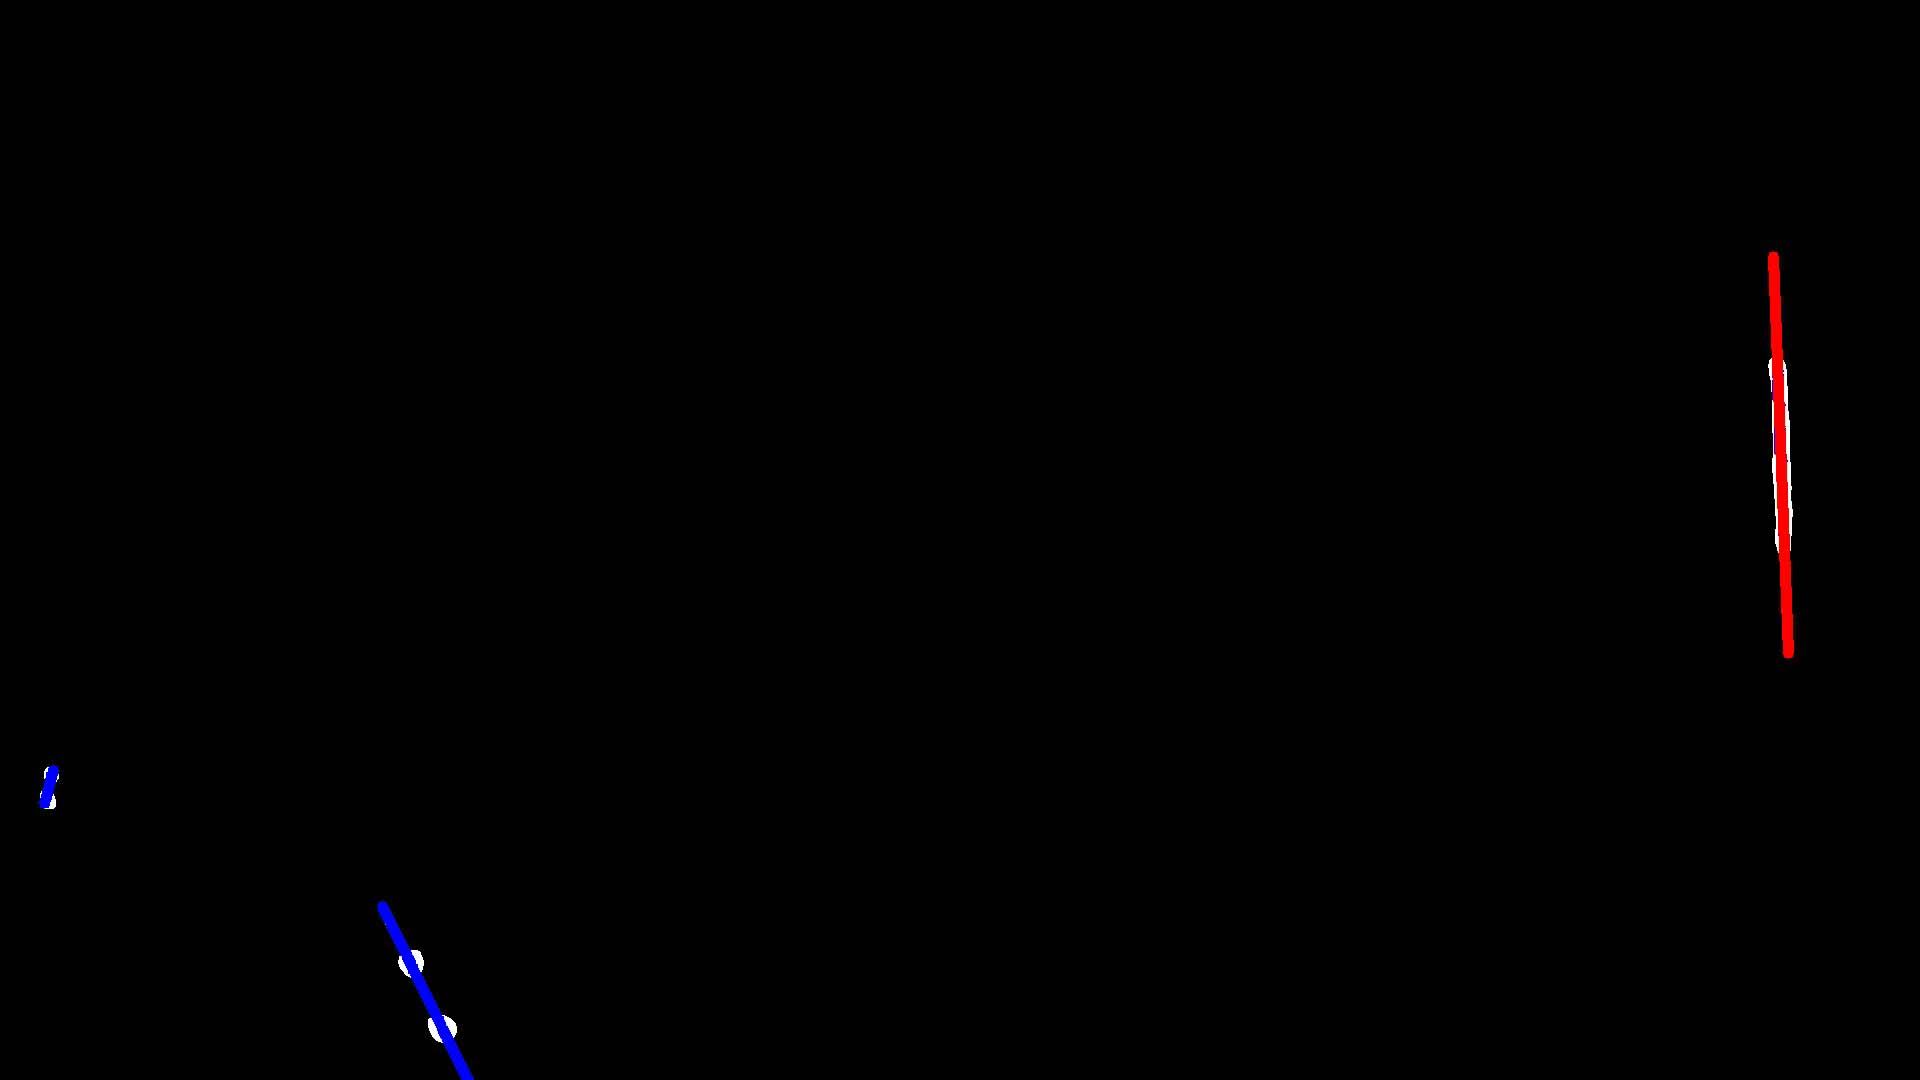
\includegraphics[width=.45\textwidth]{mask6}
	\caption{Particles identified\label{fig:mask6}}
\end{figure}

\subsection{Particle Energies}

The density of an air-isopropyl alcohol vapor mixture is 1.05 times the density of air at 20 \degree{}C \cite{isopropanol}, so at -35 \degree{}C it is $1.05 \cdot \frac{1.2754 \kilogram}{\metre^3} \cdot \frac{(-35+273) \kelvin}{(20+273) \kelvin} \cdot \frac{1 \metre^3}{1000 \kilogram} = 0.001088$ times the density of water, so particles will travel $\frac{1}{0.001088}=919$ times as far.

The field of view of the camera was around 20 cm wide, so each pixel was $\frac{20}{1920} = 0.01$ cm wide. 

The penetration depth of a beta particle in water is approximately 0.5 \centi{}\meter/\mega{}\electronvolt energy that it has \cite{penetration}, so the penetration depth in the fog is approximately 4.6 \meter/\mega{}\electronvolt.   Therefore, the energy of a beta particle, in terms of the length of its track, is 22 \electronvolt/pixel.

The penetration depth of a much heavier alpha particle in water is approximately 0.03 \centi{}\meter/\mega{}\electronvolt \cite{penetration,energies}, so its penetration depth in the fog is approximately 28 \centi{}\meter/\mega{}\electronvolt.  Therefore, the energy of an alpha particle, in terms of the length of its track, is 300 \electronvolt/pixel.

\section{Results from Test Database}

At the time of writing I've analyzed around 50 minutes of video because of difficulties in converting the video format in multi-GB files, but this still represents 731 events.  Histograms for each data value collected are presented below and color coded by particle type (red is alpha particle, blue is beta particle, muons are not distinguished), as well as selected scatterplots.  52 events, 7\% of events, are alpha particles, and 679 events, 93\%, are beta particles.  This falls in line with previous experiments.

\begin{figure}[h!]
\centering
\begin{subfigure}{.3\textwidth}
  \centering
  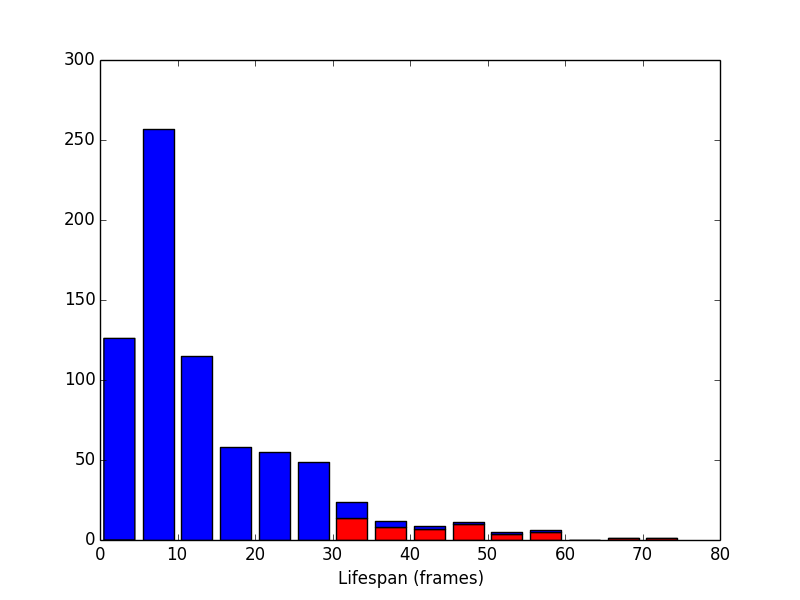
\includegraphics[width=\textwidth]{lifespan}
  \label{fig:lifespan}
  \caption{Lifespans in frames}
\end{subfigure}
\begin{subfigure}{.3\textwidth}
  \centering
  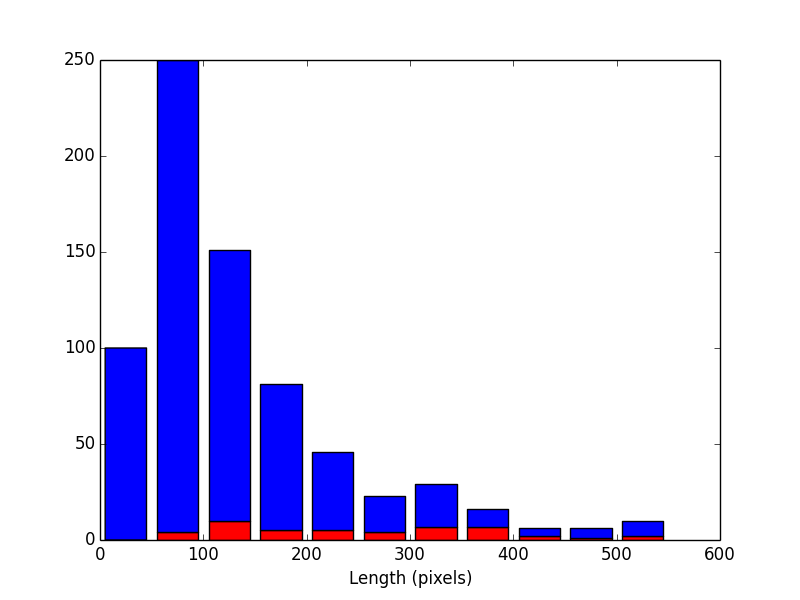
\includegraphics[width=\textwidth]{length}
  \label{fig:length}
  \caption{Lengths in pixels}
\end{subfigure}
\begin{subfigure}{.3\textwidth}
  \centering
  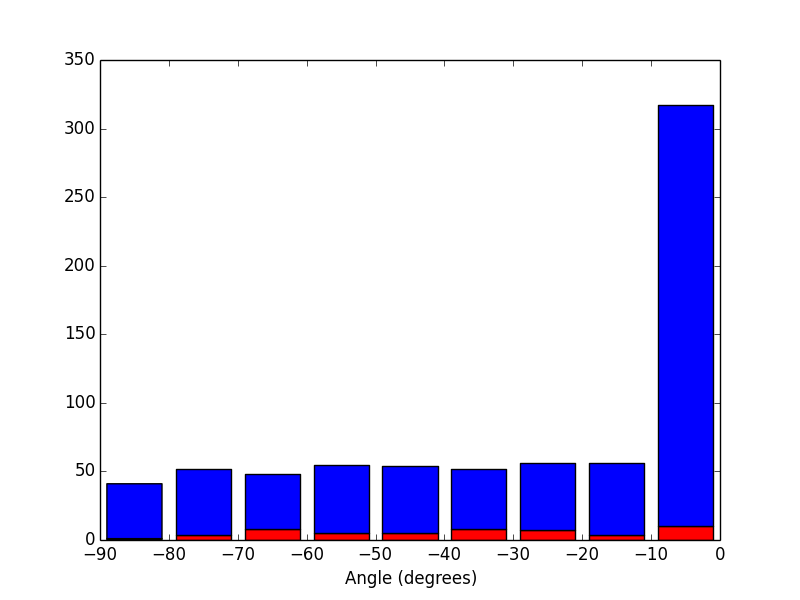
\includegraphics[width=\textwidth]{angle}
  \label{fig:angle}
  \caption{Angles in degrees}
\end{subfigure}
\label{fig:test}
\end{figure}

Beta particle tracks tended to have shorter lifespans, with a mean of 11.4 frames or 0.38 seconds and a standard deviation of 8.3 frames or 0.28 seconds, while alpha particles tended to have longer lifespans, with a mean of 44.7 frames or 1.49 seconds and a standard deviation of 13.0 frames or 0.43 seconds.  Beta particle lifespans were right-skewed, with a median of just 8.0 frames or 0.27 seconds, while alpha particle lifespans were in a roughly symmetric distribution. 

A similar, though less pronounced, pattern occurred in the particle lengths.  Beta particle lengths were again right-skewed, with a mean of 134 pixels, a standard deviation of 113 pixels, and a median of 98 pixels.  Alpha particle lengths were symmetric and greater than the beta particle lengths, with a mean of 298 pixels, a standard deviation of 183 pixels, and a median of 295 pixels.

The distribution of track angles was roughly even, except for a large spike in beta particle angles around 0, due to \texttt{minAreaRect} preferentially identifying horizontal and vertical bounding rectangles.  Surprisingly, alpha particles were more immune to this effect. 

\begin{figure}[h!]
\centering
\ContinuedFloat 
\begin{subfigure}{.3\textwidth}
  \centering
  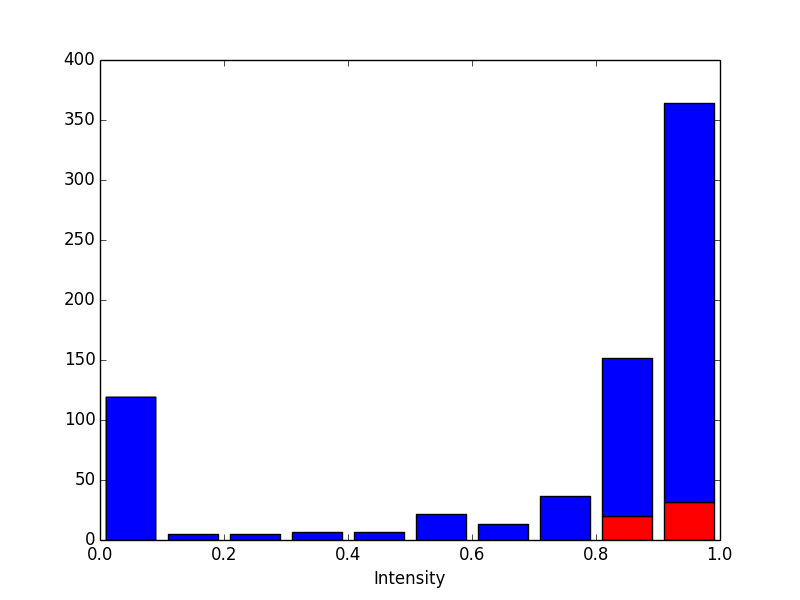
\includegraphics[width=\textwidth]{intensity}
  \label{fig:intensity}
  \caption{Intensity}
\end{subfigure}
\begin{subfigure}{.3\textwidth}
  \centering
  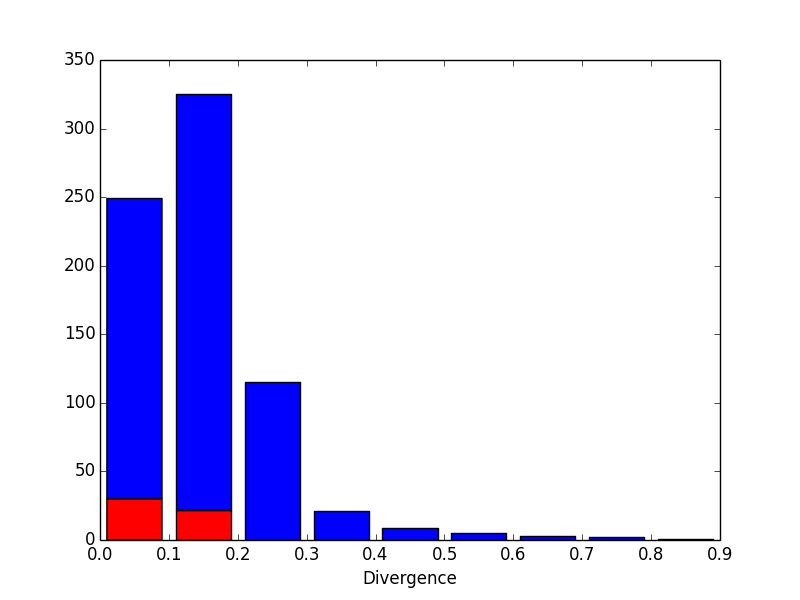
\includegraphics[width=\textwidth]{divergence}
  \label{fig:divergence}
  \caption{Divergence}
\end{subfigure}
\begin{subfigure}{.3\textwidth}
  \centering
  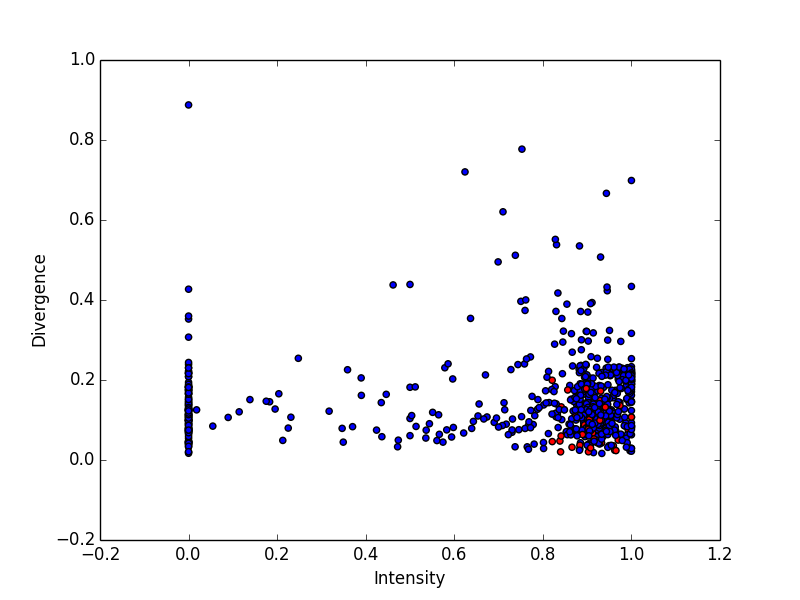
\includegraphics[width=\textwidth]{scatterid}
  \label{fig:scatterid}
  \caption{Intensity/Divergence}
\end{subfigure}
\label{fig:test}
\end{figure}

Particle intensities were heavily left-skewed, with most particles having an intensity greater than 0.8.  Similarly, particle divergences were heavily right-skewed, with most particles having a divergence less than 0.2.  Although intensity and divergence tended to have similar (though inverse) distributions, they are not correlated well.  Intensity measures the strength of the track, while divergence measures the track's curvature.

\begin{figure}[h!]
\centering
\ContinuedFloat 
\begin{subfigure}{.45\textwidth}
  \centering
  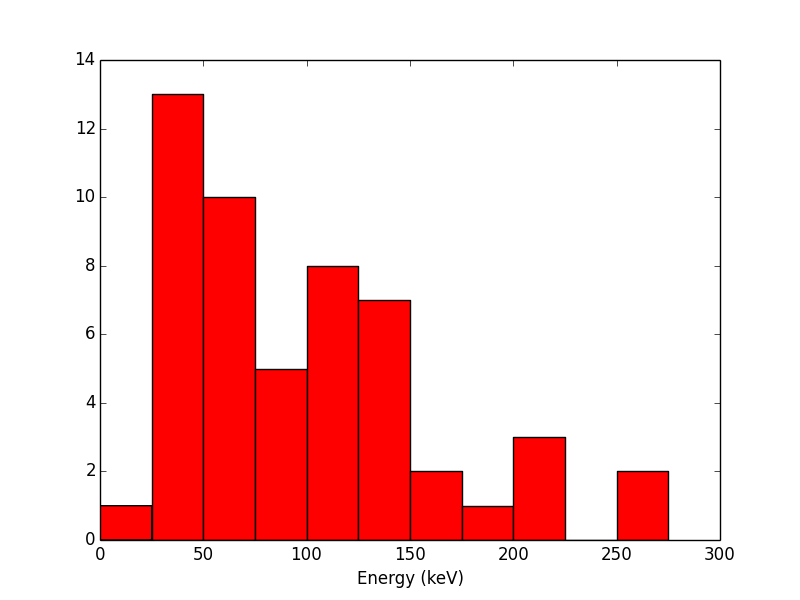
\includegraphics[width=\textwidth]{alphaenergy}
  \label{fig:alphaenergy}
  \caption{Alpha particle energies}
\end{subfigure}
\begin{subfigure}{.45\textwidth}
  \centering
  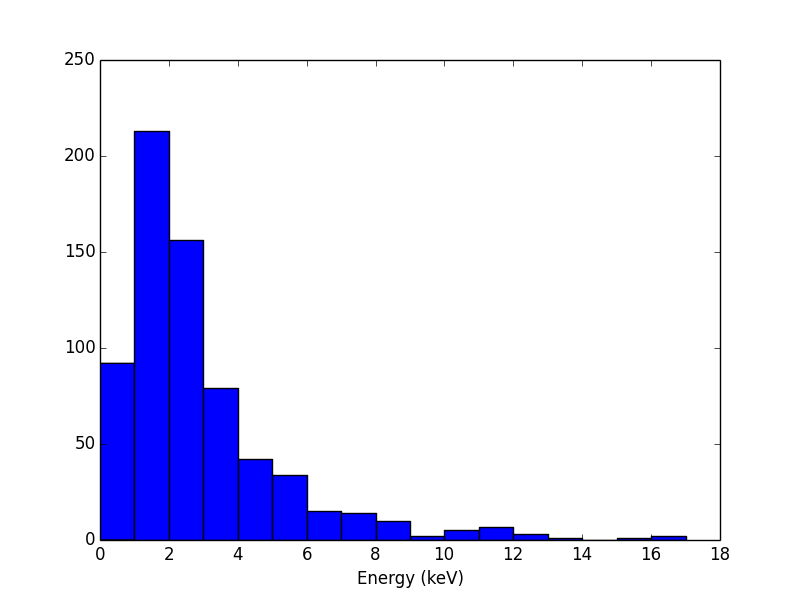
\includegraphics[width=\textwidth]{betaenergy}
  \label{fig:betaenergy}
  \caption{Beta particle energies}
\end{subfigure}
\end{figure}

Beta particle energies were right-skewed, with a mode around 1 keV and a median of 2.16 keV.  In contrast, alpha particle energies were more evenly distributed, with a median of 97.4 keV.

Alpha particle energies had a mean of 98.3 keV and a high standard deviation of 60.3 keV, while beta particles energies had a mean of 2.96 keV and a standard deviation of 2.48 keV.

\begin{figure}[h!]
\centering
\ContinuedFloat 
\begin{subfigure}{.45\textwidth}
  \centering
  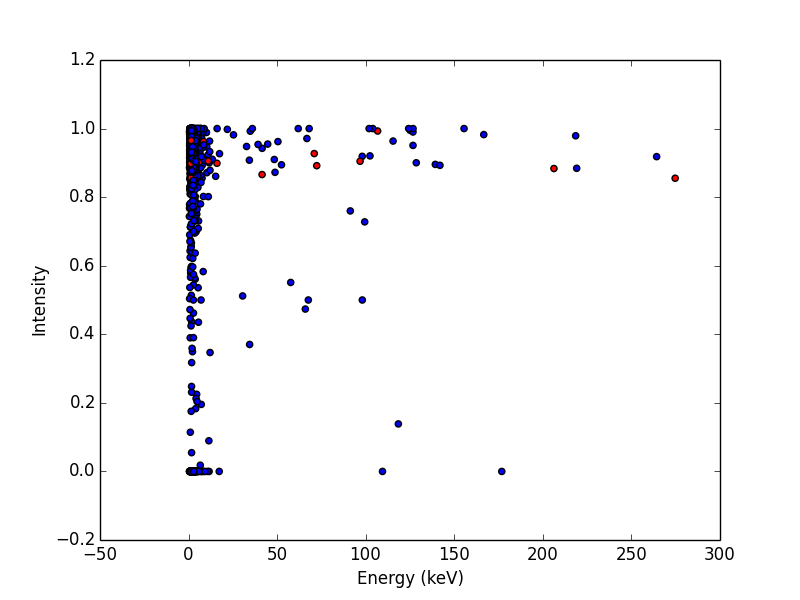
\includegraphics[width=\textwidth]{energyintensity}
  \label{fig:energyintensity}
  \caption{Energy vs. Intensity}
\end{subfigure}
\begin{subfigure}{.45\textwidth}
  \centering
  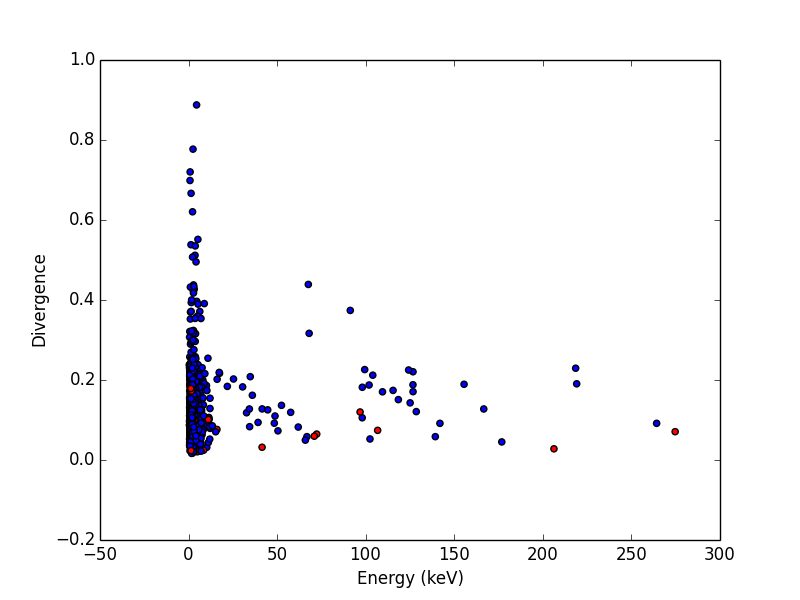
\includegraphics[width=\textwidth]{energydivergence}
  \label{fig:energydivergence}
  \caption{Energy vs. Divergence}
\end{subfigure}
\end{figure}

The particle energies had no clear correlation with either intensity or divergence.

\section{Conclusion}

Enabling automatic particle detection in cloud chambers removes a significant hurdle to widespread use of these devices in many areas of research as well as education.
  
The algorithms outlined in this paper are less sophisticated compared to other motion tracking algorithms or particle analysis programs.  This is both a drawback and a benefit: although the program is not as accurate as it could be, it can be understood and tinkered with.  The very fact that a reasonable accuracy has been achieved with such a program holds great promise for future, more complex methods of automating cloud chambers. 

\section{Continued Research}

There are some improvements, albeit time-consuming, that could be made to the current program without altering its structure.  One shortcoming is its naive line-calculation procedure.  Perhaps a better method could be linear regression on non-zero pixels within each contour.  Alternatively, more advanced methods include contour midline calculation and approximation with cubic splines.  A non-inherently-linear method for tracing track paths has another advantage in that it can fairly easily detect collisions (which will be at the points of maximum curvature).  The program does not attempt to find collisions or decay events in the tracks, but rather just the paths themselves. 
 
Other improvements could come from the video-taking procedure itself.  I used one flashlight to illuminate the track-forming region, which produced a light gradient.  Evenly illuminating the chamber, perhaps with rows of LEDs, would allow video analysis of tracks to expand to the actual frame itself instead of just analyzing the foreground mask \cite{wayne}.  This would likely improve the accuracy of the intensity, which would lend itself to an easier identification of particle type.  In addition, if a strong magnetic field were applied to the chamber, the resulting curvature of the tracks would allow an accurate calculation of particle energy, instead of the heuristics based on track length used here.   However, it is difficult to produce the required field in a small-scale experiment.

What is clear, though, is that the general detection method outlined in this paper, with fairly straightforward algorithms, can detect particle tracks in cloud chambers with good accuracy.  An automatic portable particle detector that can be made for less than 100 dollars is sure to please scientists at every level.

\begin{appendices}

\clearpage

\section{Program Listing}
\subsection{\texttt{main.py}}
\lstinputlisting{main.py}

\clearpage

\subsection{\texttt{contours.py}}
\lstinputlisting{contours.py}

\clearpage

%\section{Bibliography}
%\begin{center}References\end{center}
%
%\begin{hangparas}{2em}{1}
%Aleksandrov, A. B., Polukhina, N. G., \& Starkov, N. I. (n.d.). Methods for Image Recognition of 
%     Charged Particle Tracks in Track Detector Data Automated Processing. Intech, 213-244. 
%     
%Bertola, D., Cirilli, M., Flammer, J., Schlager, G., Schuh, S., \& Schune, P. (2004, October 16). 
%     Cloud Chamber Workshop \lbrack{}PDF\rbrack. Retrieved from https:// teachers.web.cern.ch/teachers/document/ 
%     cloud-final.pdf 
%     
%Charley, S. (2015, January 20). How to build your own particle detector. Symmetry. Retrieved from 
%     http://www.symmetrymagazine.org/article/january-2015/how-to-build-your-own-particle-detector 
%     
%Chen, Y., \& Ahmed, S. (2002). Normalized Bragg Peak Curves for Various Proton Energies in Water 
%     Phantom: A Simulation with GEANT4 Monte Carlo Code \lbrack{}PDF\rbrack. American Association of Physicists in 
%     Medicine. Retrieved from http://www.aapm.org/meetings/amos2/pdf/34-8159-78594-298.pdf 
%     
%Gupta, N.N. D., \& Ghosh, S. K. (1946). A report on the Wilson cloud chamber and its applications in 
%     physics. Review of Modern Physics, 18(2), 225-284. 
%     
%Isopropanol. (2015). In PubChem Compound Database. Retrieved from http:// pubchem.ncbi.nlm.nih.gov/ 
%     compound/isopropanol 
%     
%Langsdorf, A., Jr. (1939). A Continuously Sensitive Diffusion Cloud Chamber \lbrack{}PDF\rbrack. Review of 
%     Scientific Instruments, 10, 91-103. Retrieved from http:// hep.ucsb.edu/people/hnn/cloud/ 
%     articles/ALangsdorfRSI10\_91\_1939.pdf 
%     
%Schmidt, W. (n.d.). Cloud Chambers. Retrieved December 7, 2015, from 
%     http://www.waynesthisandthat.com/\\cloud\%20chamber.html 
%     
%Williams, T. (2008, May 31). Penetration of Different Types of Radiation. Retrieved December 8, 
%     2015, from http://www.alpharubicon.com/basicnbc/ RadiationPenetration.htm 
%     
%\end{hangparas}
%
%


\bibliography{paper}{}
\bibliographystyle{plain}

\end{appendices}

\end{document}